% !TeX program = xelatex
% !TeX TXS-program:compile = txs:///xelatex
% =====================================================================
%  BÁO CÁO TIỂU LUẬN HỌC PHẦN HỌC MÁY
%  Đề tài: Phân nhóm cổ phiếu theo mức độ đồng biến động giá phục vụ đa dạng hóa danh mục đầu tư
%  Giảng viên hướng dẫn: Thầy Nguyễn Tuấn Anh
%  Nhóm sinh viên thực hiện: Trần Phương Đoàn & Hà Văn Dũng
%  Biên dịch bằng XeLaTeX
% =====================================================================
\documentclass[12pt,a4paper,oneside,openany]{report}

% Cỡ chữ thân bài 13pt (theo quy định trình bày của bộ môn)
\makeatletter
\renewcommand\normalsize{%
  \@setfontsize\normalsize{13pt}{15.6pt}%
  \abovedisplayskip 12pt plus3pt minus7pt
  \belowdisplayskip \abovedisplayskip
  \abovedisplayshortskip 0pt plus3pt
  \belowdisplayshortskip 6.5pt plus3.5pt minus3pt}
\normalsize
\makeatother

% =====================================================================
%  (A) THÔNG TIN BÁO CÁO
% =====================================================================
\newcommand{\truong}{TRƯỜNG ĐẠI HỌC CÔNG NGHỆ THÔNG TIN VÀ TRUYỀN THÔNG}
\newcommand{\khoa}{KHOA CÔNG NGHỆ THÔNG TIN}
\newcommand{\loaibaocao}{BÁO CÁO TIỂU LUẬN}
\newcommand{\hocphan}{Học máy}
\newcommand{\lophocphan}{CNTT K22G}
\newcommand{\hocky}{Học kỳ 1, năm học 2026--2027}
\newcommand{\tendetai}{PHÂN NHÓM CỔ PHIẾU THEO MỨC ĐỘ ĐỒNG BIẾN ĐỘNG GIÁ PHỤC VỤ ĐA DẠNG HÓA DANH MỤC ĐẦU TƯ}
\newcommand{\tenbaitoan}{phân nhóm cổ phiếu}
\newcommand{\giangvien}{Thầy Nguyễn Tuấn Anh}
\newcommand{\nhom}{Nhóm 1}
\newcommand{\svAten}{Trần Phương Đoàn}
\newcommand{\svAma}{DTC235200199}
\newcommand{\svBten}{Hà Văn Dũng}
\newcommand{\svBma}{DTC235200121}
\newcommand{\diadiem}{Thái Nguyên}
\newcommand{\thoigian}{tháng 10 năm 2026}

% ---------------- Trang giấy & phông chữ ----------------
\usepackage[a4paper,left=3cm,right=2cm,top=2.5cm,bottom=2.5cm,
            headheight=16pt,headsep=0.8cm]{geometry}
\usepackage{fontspec}
\setmainfont{Times New Roman}
\setsansfont{Times New Roman}
\setmonofont{Times New Roman}
\usepackage[vietnamese]{babel}
\usepackage{setspace}
\setstretch{1.3}
\setlength{\parindent}{1cm}
\setlength{\parskip}{6pt}
\usepackage{indentfirst}

% ---------------- Gói hỗ trợ ----------------
\usepackage{amsmath,amssymb}
\usepackage{graphicx}
\graphicspath{{images/}}
\usepackage{float}
\usepackage{array,booktabs,tabularx,multirow}
\usepackage{xltabular}
\renewcommand{\arraystretch}{1.25}
\setlength{\arrayrulewidth}{0.8pt}  % Tăng độ dày nét kẻ từ 0.4pt lên 0.8pt để PDF viewer hiển thị sắc nét ở mọi mức zoom
\setlength{\extrarowheight}{1.5pt}  % Tăng đệm chiều cao hàng giúp màu nền ô không đè lên đường kẻ viền
\usepackage[table]{xcolor}
\usepackage{tikz}
\usetikzlibrary{positioning,arrows.meta,calc,fit,backgrounds}
\usepackage{caption}
\captionsetup{labelsep=period,labelfont=bf,font=normalsize,skip=6pt}
\captionsetup[table]{position=top}
\usepackage{titlesec}
\usepackage{titletoc}
\usepackage[nottoc]{tocbibind}
\usepackage{enumitem}
\setlist{nosep,leftmargin=1.6cm}
\usepackage{listings}
\usepackage{needspace}
\usepackage{cite}
\usepackage{fancyhdr}
\usepackage{xurl}
\usepackage[unicode]{hyperref}
\urlstyle{same}
\hypersetup{
  hidelinks,
  pdftitle={\tendetai},
  pdfauthor={\svAten, \svBten},
  pdfsubject={\loaibaocao\ học phần \hocphan},
  bookmarksnumbered=true,
  bookmarksopen=true,
  bookmarksopenlevel=0,
}
\newcommand{\bmchapname}{Chương}
\makeatletter
\newcommand*{\bm@prefix}{}
\let\bm@orig@writebookmark\Hy@writebookmark
\renewcommand*{\Hy@writebookmark}[5]{%
  \ifnum#4=0 \def\bm@prefix{\bmchapname\space}\else\def\bm@prefix{}\fi
  \bm@orig@writebookmark{#1}{#2}{#3}{#4}{#5}}
\renewcommand*{\Hy@numberline}[1]{\bm@prefix#1. }
\makeatother

% ---------------- Màu & định dạng mã nguồn ----------------
\definecolor{codebg}{RGB}{247,247,247}
\definecolor{codekw}{RGB}{0,51,153}
\definecolor{codecm}{RGB}{0,128,0}
\definecolor{codestr}{RGB}{163,21,21}
\definecolor{guide}{RGB}{110,110,110}
\lstdefinestyle{python}{
  language=Python,
  basicstyle=\fontspec{Times New Roman}\small\setstretch{1.0},
  backgroundcolor=\color{codebg},
  keywordstyle=\fontspec{Times New Roman}\color{codekw}\bfseries,
  commentstyle=\fontspec{Times New Roman}\color{codecm}\itshape,
  stringstyle=\fontspec{Times New Roman}\color{codestr},
  numbers=left, numberstyle=\tiny\color{guide}, numbersep=8pt,
  frame=single, rulecolor=\color{black!25},
  breaklines=true, showstringspaces=false, tabsize=4,
  xleftmargin=1.2em, framexleftmargin=1.2em,
  aboveskip=8pt, belowskip=8pt, columns=fullflexible, keepspaces=true,
}
\lstset{style=python}
\renewcommand{\lstlistingname}{Đoạn mã}
\renewcommand{\lstlistlistingname}{DANH MỤC ĐOẠN MÃ}

% ---------------- Tên gọi tiếng Việt ----------------
\addto\captionsvietnamese{%
  \renewcommand{\contentsname}{MỤC LỤC}%
  \renewcommand{\listfigurename}{DANH MỤC HÌNH ẢNH}%
  \renewcommand{\listtablename}{DANH MỤC BẢNG}%
  \renewcommand{\bibname}{TÀI LIỆU THAM KHẢO}%
  \renewcommand{\figurename}{Hình}%
  \renewcommand{\tablename}{Bảng}%
  \renewcommand{\chaptername}{Chương}%
  \renewcommand{\appendixname}{Phụ lục}%
}

% ---------------- Đầu trang & chân trang ----------------
\pagestyle{fancy}
\fancyhf{}
\fancyhead[L]{\small\itshape Báo cáo tiểu luận học phần \hocphan}
\fancyhead[R]{\small\itshape\nouppercase{\leftmark}}
\fancyfoot[C]{\thepage}
\renewcommand{\headrulewidth}{0.4pt}
\renewcommand{\chaptermark}[1]{\markboth{\chaptertitlename~\thechapter. #1}{}}
\fancypagestyle{plain}{\fancyhf{}\fancyfoot[C]{\thepage}\renewcommand{\headrulewidth}{0pt}}

% ---------------- Định dạng tiêu đề ----------------
\titleformat{\chapter}[display]
  {\filcenter\bfseries\fontsize{14}{18}\selectfont}
  {\MakeUppercase{\chaptertitlename}~\thechapter}{4pt}{\MakeUppercase}
\titlespacing*{\chapter}{0pt}{0pt}{18pt}

\titleformat{\section}
  {\bfseries\fontsize{14}{18}\selectfont}{\thesection.}{0.5em}{}
\titlespacing*{\section}{0pt}{12pt}{6pt}

\titleformat{\subsection}
  {\bfseries\fontsize{13}{17}\selectfont}{\thesubsection.}{0.5em}{}
\titlespacing*{\subsection}{0pt}{10pt}{6pt}

\setcounter{secnumdepth}{3}
\titleformat{\subsubsection}
  {\bfseries\itshape\fontsize{13}{17}\selectfont}{\thesubsubsection.}{0.5em}{}
\titlespacing*{\subsubsection}{0pt}{8pt}{4pt}

% ---------------- Mục lục & danh mục ----------------
\setcounter{tocdepth}{2}
\newcommand{\tocchapname}{Chương}
\titlecontents{chapter}[0pt]{\addvspace{6pt}\bfseries}
  {\tocchapname~\thecontentslabel.\enspace}{}{\titlerule*[0.6pc]{.}\contentspage}
\titlecontents{section}[1.5em]{}
  {\thecontentslabel.\enspace}{}{\titlerule*[0.6pc]{.}\contentspage}
\titlecontents{subsection}[3em]{}
  {\thecontentslabel.\enspace}{}{\titlerule*[0.6pc]{.}\contentspage}
\titlecontents{figure}[0pt]{}
  {\figurename~\thecontentslabel.\enspace}{}{\titlerule*[0.6pc]{.}\contentspage}
\titlecontents{table}[0pt]{}
  {\tablename~\thecontentslabel.\enspace}{}{\titlerule*[0.6pc]{.}\contentspage}

% ---------------- Lệnh tiện ích ----------------
\newcommand{\unnumberedchapter}[1]{%
  \chapter*{#1}\phantomsection\addcontentsline{toc}{chapter}{#1}\markboth{#1}{}}
\newcommand{\khunghinh}[3]{%
  \begin{tikzpicture}
    \draw[dashed,thick,black!40,fill=black!3] (0,0) rectangle (#1,#2);
    \node[text width=0.8*#1,align=center,font=\itshape\color{guide}]
      at ($(0,0)!0.5!(#1,#2)$) {#3};
  \end{tikzpicture}}
\newcommand{\dongcham}[1]{\par\noindent\foreach \i in {1,...,#1}{\makebox[\linewidth]{\dotfill}\\[4pt]}}

% =====================================================================
\begin{document}

% =====================================================================
%  TRANG BÌA
% =====================================================================
\begin{titlepage}
  \begin{tikzpicture}[remember picture,overlay]
    \draw[line width=2.2pt]
      ($(current page.north west)+(2.4cm,-1.6cm)$) rectangle
      ($(current page.south east)+(-1.4cm,1.6cm)$);
    \draw[line width=0.6pt]
      ($(current page.north west)+(2.55cm,-1.75cm)$) rectangle
      ($(current page.south east)+(-1.55cm,1.75cm)$);
  \end{tikzpicture}\par\vspace*{-\baselineskip}
  \centering\setstretch{1.2}
  {\fontsize{13}{18}\selectfont\bfseries \truong\par}
  {\fontsize{14}{18}\selectfont\bfseries \khoa\par}
  \vspace{2pt}\rule{0.35\textwidth}{0.8pt}\par
  \vspace{1.2cm}
  \IfFileExists{images/logo_ictu.jpg}
    {
\includegraphics[width=3.5cm]{logo_ictu.jpg}}
    {\khunghinh{3.5cm}{3.5cm}{Logo\\ICTU}}\par
  \vspace{1.0cm}
  {\fontsize{18}{24}\selectfont\bfseries \loaibaocao\par}
  \vspace{4pt}
  {\fontsize{15}{20}\selectfont\bfseries HỌC PHẦN: \MakeUppercase{\hocphan}\par}
  \vspace{0.8cm}
  {\fontsize{13}{17}\selectfont ĐỀ TÀI:\par}
  \vspace{4pt}
  {\fontsize{16}{22}\selectfont\bfseries \tendetai\par}
  \vfill
  \begin{tabular}{@{}l@{\hspace{0.6cm}}l@{}}
    \textbf{Giảng viên hướng dẫn:} & \giangvien \\
    \textbf{Lớp học phần:}         & \lophocphan \\
    \textbf{Nhóm thực hiện:}       & \nhom \\
                                   & \svAten\ -- \svAma \\
                                   & \svBten\ -- \svBma \\
  \end{tabular}\par
  \vspace{1.5cm}
  {\bfseries \diadiem, \thoigian\par}
\end{titlepage}

% =====================================================================
%  PHẦN ĐẦU (đánh số trang La Mã)
% =====================================================================
\pagenumbering{roman}
\pagestyle{plain}

% ---------------- Nhận xét của giảng viên ----------------
\chapter*{NHẬN XÉT CỦA GIẢNG VIÊN}
\noindent\textbf{1. Về hình thức và bố cục báo cáo:}
\dongcham{3}
\noindent\textbf{2. Về nội dung và kết quả thực hiện:}
\dongcham{5}
\noindent\textbf{3. Về tinh thần, thái độ làm việc của nhóm:}
\dongcham{3}
\noindent\textbf{4. Điểm đánh giá:}
\begin{center}
  \begin{tabular}{|>{\centering\arraybackslash}p{1.2cm}|p{5.5cm}|>{\centering\arraybackslash}p{2.6cm}|>{\centering\arraybackslash}p{2.6cm}|}
    \hline
    \rowcolor{black!8}\textbf{STT} & \textbf{Họ và tên sinh viên} & \textbf{Điểm số} & \textbf{Điểm chữ} \\ \hline
    1 & \svAten & & \\ \hline
    2 & \svBten & & \\ \hline
  \end{tabular}
\end{center}
\vspace{0.6cm}
\hfill
\begin{minipage}{0.45\textwidth}
  \centering
  \textit{\diadiem, ngày \dots\ tháng \dots\ năm \dots}\\
  \textbf{Giảng viên}\\
  \textit{(Ký và ghi rõ họ tên)}\\[1.8cm]
  \giangvien
\end{minipage}

% ---------------- Lời cam đoan ----------------
\unnumberedchapter{LỜI CAM ĐOAN}

Chúng em xin cam đoan báo cáo tiểu luận ``\textit{\tendetai}'' là kết quả làm việc nghiêm túc của nhóm dưới sự định hướng chuyên môn của \giangvien. Mọi dữ liệu thu thập, các quyết định tiền xử lý, công thức chuyển đổi mêtric khoảng cách và số liệu thực nghiệm trình bày trong báo cáo đều được trích xuất hoàn toàn trung thực từ hệ thống mã nguồn Python và 5 sổ tay Jupyter Notebook của nhóm; tất cả các kết quả thực nghiệm đều có khả năng chạy lại và tái hiện độc lập.

\textbf{Khai báo sử dụng công cụ AI tạo sinh:}
Trong quá trình thực hiện dự án, nhóm có sử dụng các mô hình ngôn ngữ lớn (Gemini, Claude) với vai trò trợ lý hỗ trợ kỹ thuật: tra cứu tài liệu học thuật về lý thuyết ma trận ngẫu nhiên (RMT), tối ưu hóa cú pháp mã nguồn Python vẽ biểu đồ khoa học, và hỗ trợ rà soát kiểm tra lỗi định dạng văn bản LaTeX. Toàn bộ các phân tích thống kê, logic phát biểu bài toán, quy tắc điền khuyết chống rò rỉ dữ liệu, việc kiểm chứng toán học mêtric Mantegna và viết nội dung báo cáo đều do các thành viên trong nhóm trực tiếp nghiên cứu, lập trình và chịu trách nhiệm giải trình.

Nếu phát hiện có bất kỳ sự sao chép trái phép hay gian lận học thuật nào, nhóm chúng em xin hoàn toàn chịu mọi hình thức kỷ luật trước giảng viên và nhà trường.

\vspace{0.6cm}
\hfill
\begin{minipage}{0.5\textwidth}
  \centering
  \textit{\diadiem, ngày \dots\ tháng 10 năm 2026}\\
  \textbf{Nhóm sinh viên thực hiện}\\
  \textit{(Ký và ghi rõ họ tên)}\\[2cm]
  \begin{tabular}{@{}c@{\hspace{1.5cm}}c@{}}
    \svAten & \svBten
  \end{tabular}
\end{minipage}

% ---------------- Lời cảm ơn ----------------
\unnumberedchapter{LỜI CẢM ƠN}

Nhóm chúng em xin bày tỏ lòng biết ơn sâu sắc và chân thành nhất tới \textbf{\giangvien}, người đã tận tình hướng dẫn, trang bị những nền tảng lý thuyết vững chắc về bộ môn Học máy và trực tiếp định hướng cho nhóm tiếp cận một đề tài mang tính liên ngành cao giữa Trí tuệ nhân tạo và Tài chính định lượng (Quantitative Finance). Sự chỉ dẫn khoa học, những nhận xét sâu sắc của thầy trong các buổi học trên lớp và các tiêu chí chấm điểm chuẩn mực đã giúp nhóm định hình rõ ràng phương pháp tiếp cận đúng đắn, xây dựng quy trình tiền xử lý dữ liệu chặt chẽ và phòng chống triệt để các rủi ro rò rỉ dữ liệu trong chuỗi thời gian tài chính.

Nhóm cũng xin chân thành cảm ơn các thầy cô giáo trong Khoa Công nghệ Thông tin -- Trường Đại học Công nghệ Thông tin và Truyền thông đã tạo điều kiện học tập thuận lợi, xây dựng chương trình đào tạo hiện đại giúp sinh viên có đủ kiến thức và kỹ năng thực hành để hoàn thành giai đoạn đầu tiên của dự án. 

Mặc dù nhóm đã nỗ lực hết mình để khảo sát, tiền xử lý và thiết lập không gian dữ liệu một cách khoa học nhất, song do thời gian và kiến thức còn hạn chế, báo cáo chắc chắn khó tránh khỏi những thiếu sót. Chúng em rất mong tiếp tục nhận được những ý kiến đóng góp, chỉ bảo quý báu của thầy để nhóm hoàn thiện tốt hơn nữa trong các giai đoạn huấn luyện mô hình (Bài kiểm tra 2) và ứng dụng thực tiễn (Bài kiểm tra 3) tiếp theo.

\vspace{0.4cm}
\hfill\textit{Nhóm sinh viên thực hiện}

% ---------------- Bảng phân công ----------------
\unnumberedchapter{BẢNG PHÂN CÔNG NHIỆM VỤ}

\begin{center}
\begin{tabularx}{\textwidth}{|>{\centering\arraybackslash}p{1cm}|p{3.2cm}|X|>{\centering\arraybackslash}p{2.3cm}|}
  \hline
  \rowcolor{black!8}\textbf{STT} & \textbf{Họ và tên} & \textbf{Nhiệm vụ phụ trách} & \textbf{Mức độ hoàn thành} \\ \hline
  1 & \svAten\newline (\svAma) &
    -- Thu thập dữ liệu thô 100 mã VN100 qua API (\texttt{nb01})\newline
    -- Phát hiện và xử lý vấn đề chất lượng: lọc 2 mã thiếu, khử 68 ngày nghỉ lễ, điền khuyết Forward-fill (\texttt{nb02})\newline
    -- Tính toán ma trận tương quan Pearson và thiết lập mêtric khoảng cách Mantegna, kiểm định bất đẳng thức tam giác (\texttt{nb04})\newline
    -- Viết nội dung Chương 2 và mục tiền xử lý dữ liệu Chương 3 & 100\% \\ \hline
  2 & \svBten\newline (\svBma) &
    -- Trích chọn chuỗi lợi suất logarit, kiểm định tính dừng và phân bố đuôi béo Fat-tails, Jarque-Bera (\texttt{nb03})\newline
    -- Thiết kế chiến lược phân chia Train/Test theo chu kỳ thị trường dựa trên lý thuyết ma trận ngẫu nhiên RMT (\texttt{nb05})\newline
    -- Xây dựng từ điển dữ liệu, khảo sát thống kê rủi ro -- lợi suất, đối chiếu phân ngành ICB\newline
    -- Viết nội dung Chương 1 và mục phân chia dữ liệu Chương 3 & 100\% \\ \hline
\end{tabularx}
\end{center}

% ---------------- Mục lục, danh mục ----------------
\begingroup\setstretch{1.1}\tableofcontents\endgroup
\listoffigures
\listoftables

% ---------------- Danh mục từ viết tắt ----------------
\unnumberedchapter{DANH MỤC TỪ VIẾT TẮT}

\begin{center}
\begin{tabularx}{\textwidth}{|>{\centering\arraybackslash}p{1cm}|p{2.5cm}|X|}
  \hline
  \rowcolor{black!8}\textbf{STT} & \textbf{Viết tắt} & \textbf{Thuật ngữ đầy đủ và ý nghĩa} \\ \hline
  1 & ARI   & Adjusted Rand Index -- Chỉ số Rand điều chỉnh (đo độ ổn định phân cụm) \\ \hline
  2 & CCC   & Cophenetic Correlation Coefficient -- Hệ số tương quan Cophenetic \\ \hline
  3 & CVaR  & Conditional Value at Risk -- Giá trị rủi ro có điều kiện \\ \hline
  4 & EDA   & Exploratory Data Analysis -- Phân tích khám phá dữ liệu \\ \hline
  5 & HOSE  & Ho Chi Minh Stock Exchange -- Sở Giao dịch Chứng khoán TP. Hồ Chí Minh \\ \hline
  6 & ICB   & Industry Classification Benchmark -- Chuẩn phân ngành công nghiệp quốc tế \\ \hline
  7 & MDD   & Maximum Drawdown -- Mức sụt giảm vốn tối đa \\ \hline
  8 & ML    & Machine Learning -- Học máy \\ \hline
  9 & MPT   & Modern Portfolio Theory -- Lý thuyết danh mục đầu tư hiện đại Markowitz \\ \hline
  10 & OOS   & Out-of-Sample -- Ngoài mẫu (tập kiểm thử) \\ \hline
  11 & PCA   & Principal Component Analysis -- Phân tích thành phần chính \\ \hline
  12 & RMT   & Random Matrix Theory -- Lý thuyết ma trận ngẫu nhiên \\ \hline
  13 & VaR   & Value at Risk -- Giá trị rủi ro danh mục \\ \hline
  14 & VN100 & Chỉ số 100 cổ phiếu vốn hóa và thanh khoản hàng đầu thị trường Việt Nam \\ \hline
\end{tabularx}
\end{center}

% =====================================================================
%  PHẦN NỘI DUNG (đánh số trang Ả Rập)
% =====================================================================
\clearpage
\pagenumbering{arabic}
\pagestyle{fancy}

% =====================================================================
%  MỞ ĐẦU
% =====================================================================
\unnumberedchapter{MỞ ĐẦU}

\section*{1. Lý do chọn đề tài}
Trong thị trường tài chính, đa dạng hóa danh mục đầu tư là nguyên lý cốt lõi giúp nhà đầu tư giảm thiểu rủi ro phi hệ thống (rủi ro riêng lẻ của từng doanh nghiệp) mà không làm suy giảm lợi suất kỳ vọng. Theo Lý thuyết Danh mục Đầu tư Hiện đại (Modern Portfolio Theory -- MPT) của Harry Markowitz (1952), hiệu quả phân tán rủi ro phụ thuộc trực tiếp vào hệ số tương quan giữa các tài sản trong danh mục: khi nắm giữ các cổ phiếu có mức độ tương quan thấp hoặc biến động ngược chiều, phương sai tổng thể của danh mục sẽ giảm đáng kể.

Tuy nhiên, trong thực tế đầu tư, các phương pháp phân bổ tài sản truyền thống thường dựa vào phân loại ngành hành chính (như chuẩn phân ngành ICB, GICS) hoặc ước lượng ma trận hiệp phương sai trực tiếp trên quy mô lớn. Cách tiếp cận này bộc lộ hai nhược điểm nghiêm trọng:
\begin{enumerate}
  \item \textit{Tính chủ quan của phân loại ngành:} Hai cổ phiếu thuộc cùng một ngành danh nghĩa (ví dụ: nhóm Bất động sản) có thể có cấu trúc đòn bẩy tài chính và tính nhạy cảm dòng tiền rất khác nhau; ngược lại, các cổ phiếu thuộc hai ngành khác nhau (ví dụ: Thép và Bất động sản xây dựng) lại có thể đồng biến động giá rất mạnh do liên kết chuỗi cung ứng.
  \item \textit{Sự nhiễu loạn ma trận tương quan quy mô lớn:} Khi số lượng tài sản $N$ lớn, việc tối ưu hóa danh mục theo Markowitz đòi hỏi nghịch đảo ma trận hiệp phương sai, dẫn đến sự bất ổn định số học và khuếch đại sai số ước lượng (hiện tượng Markowitz Curse).
\end{enumerate}

Sự kết hợp giữa các thuật toán Học máy không giám sát (Unsupervised Machine Learning), cụ thể là các thuật toán phân cụm (Clustering), với các độ đo khoảng cách tài chính phi tuyến mở ra hướng tiếp cận ưu việt. Bằng cách phân nhóm cổ phiếu dựa trên chính mức độ đồng biến động giá lịch sử thực tế thay vì nhãn ngành chủ quan, mô hình học máy cho phép bóc tách cấu trúc vi mô của thị trường, tìm ra các nhóm cổ phiếu độc lập thực sự để phục vụ chiến lược đa dạng hóa danh mục đầu tư hiệu quả.

\section*{2. Mục tiêu và nhiệm vụ nghiên cứu}
Báo cáo tập trung giải quyết toàn diện các yêu cầu về khảo sát bài toán, thu thập, tiền xử lý dữ liệu và thiết lập không gian mêtric cho mô hình học máy phục vụ phân nhóm cổ phiếu và đa dạng hóa danh mục:
\begin{itemize}
  \item \textbf{Phát biểu chuẩn xác bài toán học máy:} Xác định rõ nhiệm vụ học máy không giám sát, đơn vị mẫu 98 mã VN100, đầu vào ma trận khoảng cách đồng biến động và đầu ra cấu trúc phân cụm; chuyển đổi mục tiêu tài chính sang các chỉ số định lượng đo lường được.
  \item \textbf{Thu thập và mô tả dữ liệu toàn diện:} Xây dựng đường ống thu thập tự động dữ liệu giá lịch sử của 100 cổ phiếu thành phần rổ VN100 giai đoạn 2022--2026; lập từ điển dữ liệu tài chính và metadata phân ngành ICB.
  \item \textbf{Khảo sát thống kê và phân tích cấu trúc dữ liệu:} Thực hiện phân tích khám phá dữ liệu (EDA), phân tích phân bố lợi suất logarit, kiểm định thống kê hiện tượng đuôi béo (Fat-tails) và phân tích không gian lợi suất -- rủi ro.
  \item \textbf{Định lượng và xử lý triệt để các vấn đề chất lượng dữ liệu:} Phát hiện và loại bỏ các mã thiếu hụt dữ liệu niên yết lớn, chuẩn hóa lịch giao dịch sàn HOSE, điền khuyết bằng phương pháp Forward-fill bảo toàn tính nhân quả và loại bỏ hoàn toàn nguy cơ rò rỉ dữ liệu tương lai (Look-ahead bias).
  \item \textbf{Thiết lập không gian khoảng cách mêtric và phân chia Train/Test:} Phân tích nhược điểm của khoảng cách Euclid, chuyển đổi hệ số tương quan Pearson sang khoảng cách Mantegna thỏa mãn 4 tiên đề mêtric; phân tách ranh giới tập Train (2022--2024) và Test (2025--2026) theo chu kỳ thị trường dựa trên cơ sở Lý thuyết Ma trận Ngẫu nhiên (RMT).
\end{itemize}

\section*{3. Đối tượng và phạm vi nghiên cứu}
\begin{itemize}
  \item \textbf{Không gian mẫu nghiên cứu:} 100 cổ phiếu thuộc rổ chỉ số VN100 niêm yết trên Sở Giao dịch Chứng khoán TP. Hồ Chí Minh (HOSE), đại diện cho hơn 90\% giá trị vốn hóa và 85\% thanh khoản toàn thị trường chứng khoán Việt Nam.
  \item \textbf{Phạm vi thời gian:} Giai đoạn 5 năm từ ngày 01/01/2022 đến ngày 23/10/2026, trải qua đầy đủ các giai đoạn thị trường đặc thù: sụt giảm sâu (Downtrend 2022), phục hồi tích lũy (2023--2024) và phân hóa đi ngang (2025--2026).
  \item \textbf{Dữ liệu sử dụng:} Chuỗi giá đóng cửa điều chỉnh (\texttt{adj\_close}) hàng ngày đã xử lý quyền chia cổ tức và phát hành thêm, cùng chuỗi lợi suất logarit liên tục.
\end{itemize}

\section*{4. Phương pháp thực hiện}
Đề tài sử dụng ngôn ngữ lập trình Python 3.12 cùng các thư viện khoa học dữ liệu chuẩn mực (\texttt{numpy}, \texttt{pandas}, \texttt{scipy}, \texttt{scikit-learn}, \texttt{matplotlib}, \texttt{seaborn}). Toàn bộ quy trình thực nghiệm được cấu trúc hóa thành 5 sổ tay Jupyter Notebook độc lập, có khả năng thực thi tuần tự và kiểm chứng kết quả trực tiếp:
\begin{itemize}
  \item \texttt{01\_data\_collection\_prep.ipynb}: Thu thập dữ liệu thô 100 mã VN100 và metadata ngành.
  \item \texttt{02\_data\_preprocessing.ipynb}: Lọc mã thiếu, khử ngày nghỉ lễ và điền khuyết Forward-fill.
  \item \texttt{03\_feature\_extraction\_returns.ipynb}: Trích chọn lợi suất logarit, kiểm định Jarque-Bera.
  \item \texttt{04\_correlation\_distance.ipynb}: Xây dựng ma trận tương quan Pearson và khoảng cách Mantegna.
  \item \texttt{05\_train\_test\_split.ipynb}: Phân chia tập Train/Test theo thời gian và xuất bản ma trận huấn luyện.
\end{itemize}

\section*{5. Bố cục báo cáo}
Nội dung báo cáo được trình bày trong 3 chương trọng tâm:
\begin{itemize}
  \item \textbf{Chương 1. Xác định bài toán học máy và cơ sở lý thuyết:} Phát biểu bài toán theo Mitchell, bảng mục tiêu -- chỉ số thành công, cơ sở không gian khoảng cách Mantegna và phương pháp luận đánh giá chuỗi thời gian.
  \item \textbf{Chương 2. Thu thập và khảo sát thống kê dữ liệu:} Nguồn gốc dữ liệu, từ điển đặc trưng tài chính, phân tích phân bố đuôi béo của lợi suất, không gian rủi ro -- lợi suất và ma trận tương quan Pearson giữa 98 cổ phiếu.
  \item \textbf{Chương 3. Tiền xử lý dữ liệu và chuẩn bị cho mô hình:} Định lượng vấn đề chất lượng, phương pháp xử lý Forward-fill, so sánh trước -- sau, chiến lược phân chia Train/Test theo chu kỳ thị trường và nguyên tắc chống rò rỉ dữ liệu.
\end{itemize}
Cuối báo cáo là phần Kết luận, Bảng tự đánh giá theo 10 tiêu chí chấm điểm của giảng viên, Danh mục tài liệu tham khảo và các Phụ lục hướng dẫn thực nghiệm.

% =====================================================================
%  CHƯƠNG 1
% =====================================================================
\chapter{Xác định bài toán học máy và cơ sở lý thuyết}
\label{chap:xacdinhbaitoan}

\section{Bối cảnh thực tiễn và bài toán đa dạng hóa danh mục}
Trong quản lý danh mục đầu tư theo trường phái hiện đại của Harry Markowitz \cite{markowitz1952}, phương sai của một danh mục gồm $N$ tài sản với các tỷ trọng phân bổ $w = [w_1, w_2, \dots, w_N]^T$ ($\sum_{i=1}^N w_i = 1$) được xác định bởi công thức:
\begin{equation}
  \sigma_p^2 = \sum_{i=1}^N w_i^2 \sigma_i^2 + 2 \sum_{i=1}^{N} \sum_{j < i} w_i w_j \sigma_i \sigma_j \rho_{ij}
  \label{eq:markowitz}
\end{equation}
Trong đó $\sigma_i, \sigma_j$ là độ lệch chuẩn (đo lường rủi ro biến động) của tài sản $i$ và $j$, còn $\rho_{ij} \in [-1, 1]$ là hệ số tương quan giữa hai chuỗi lợi suất.

Từ phương trình (\ref{eq:markowitz}), có thể thấy số lượng thành phần hiệp phương sai tăng theo cấp số bậc hai $N(N-1)/2$. Khi các tài sản có hệ số tương quan đồng pha mạnh ($\rho_{ij} \to 1$), rủi ro của danh mục xấp xỉ bằng bình quân gia quyền rủi ro các tài sản đơn lẻ, triệt tiêu hoàn toàn lợi ích của việc đa dạng hóa. Ngược lại, nếu nhóm các tài sản được lựa chọn có hệ số tương quan thấp ($\rho_{ij} \to 0$) hoặc ngược pha ($\rho_{ij} < 0$), thành phần thứ hai trong phương trình (\ref{eq:markowitz}) sẽ tiệm cận về 0 hoặc mang giá trị âm, giúp giảm mạnh độ biến động tổng thể $\sigma_p$ của danh mục.

Do đó, vấn đề cốt lõi của bài toán đầu tư thực tế là: \textit{Làm thế nào để phân nhóm tự động hàng trăm cổ phiếu trên thị trường thành các cụm có tính chất đồng biến động cao trong nội bộ cụm, nhưng hoàn toàn độc lập hoặc phân kỳ giữa các cụm khác nhau?} Giải quyết được bài toán này sẽ cung cấp cơ sở dữ liệu định lượng vững chắc để nhà đầu tư chỉ cần chọn ra các đại diện ưu tú từ các cụm khác nhau, thiết lập một danh mục đa dạng hóa tối ưu mà không bị lệ thuộc vào định kiến chủ quan của nhãn ngành truyền thống.

Quy trình thực hiện tổng quát của đề tài được mô tả trực quan trong Hình~\ref{fig:quytrinh}.

\begin{figure}[H]
  \centering
  \begin{tikzpicture}[
      node distance=0.45cm,
      buoc/.style={draw,rounded corners=3pt,fill=black!5,minimum height=1.1cm,
                   text width=1.9cm,align=center,font=\small},
      buochientai/.style={draw,rounded corners=3pt,fill=blue!10,draw=blue!80,line width=1pt,minimum height=1.1cm,
                   text width=1.9cm,align=center,font=\small\bfseries},
      mui/.style={-{Stealth[length=2.5mm]},thick}]
    \node[buochientai] (b1) {Phát biểu\\bài toán};
    \node[buochientai,right=of b1] (b2) {Thu thập\\dữ liệu};
    \node[buochientai,right=of b2] (b3) {Tiền xử lý\\\& Mêtric};
    \node[buoc,right=of b3] (b4) {Huấn luyện\\phân cụm};
    \node[buoc,right=of b4] (b5) {Đánh giá\\\& ARI};
    \node[buoc,below=0.9cm of b4] (b6) {Tối ưu \&\\Đối chiếu ICB};
    \node[buoc,below=0.9cm of b2] (b7) {Đa dạng hóa\\\& Backtest};
    \draw[mui] (b1) -- (b2);
    \draw[mui] (b2) -- (b3);
    \draw[mui] (b3) -- (b4);
    \draw[mui] (b4) -- (b5);
    \draw[mui] (b5) |- (b6);
    \draw[mui] (b6) -- (b4);
    \draw[mui] (b6) -- (b7);
  \end{tikzpicture}
  \caption{Quy trình tổng thể dự án học máy (các khối tô màu xanh đại diện cho các bước đã hoàn thành)}
  \label{fig:quytrinh}
\end{figure}

\section{Phát biểu bài toán học máy theo Mitchell}
Để chuyển bài toán thực tế thành bài toán kỹ thuật giải quyết được bằng học máy, nhóm mô hình hóa bài toán theo định nghĩa hình thức của Tom Mitchell \cite{mitchell1997} với bộ ba $(T, E, P)$:
\begin{itemize}
  \item \textbf{Loại bài toán học máy:} Học không giám sát (Unsupervised Learning) -- Cụ thể là Phân cụm chuỗi thời gian tài chính (Financial Time-Series Clustering).
  \item \textbf{Nhiệm vụ $T$ (Task):} Phân chia tập hợp $N = 98$ cổ phiếu rổ VN100 thành $k$ cụm rời nhau $C = \{C_1, C_2, \dots, C_k\}$ dựa trên ma trận khoảng cách đồng biến động giá lịch sử, sao cho:
  \begin{equation}
    \forall i, j \in C_m \implies d(i, j) \text{ nhỏ nhất}; \quad \forall i \in C_m, l \in C_p \ (m \ne p) \implies d(i, l) \text{ lớn nhất}
  \end{equation}
  \item \textbf{Kinh nghiệm $E$ (Experience):} Dữ liệu chuỗi thời gian giá đóng cửa điều chỉnh và chuỗi lợi suất logarit hàng ngày của 98 cổ phiếu trên sàn HOSE trong giai đoạn In-Sample từ 01/01/2022 đến 31/12/2024 (gồm 739 phiên giao dịch tập Train).
  \item \textbf{Độ đo hiệu năng $P$ (Performance Measure):}
  \begin{enumerate}
    \item \textit{Độ đo hình học nội bộ:} Hệ số Silhouette Score ($s_i \in [-1, 1]$) đo lường mức độ gắn kết nội cụm và phân tách ngoại cụm; Hệ số tương quan Cophenetic (CCC) đo độ trung thực của cây phân cấp so với ma trận khoảng cách gốc.
    \item \textit{Độ đo tính bền vững qua thời gian:} Chỉ số Adjusted Rand Index (ARI) giữa cấu trúc cụm học được trên tập Train so với các giai đoạn thị trường kiểm thử Out-of-Sample.
    \item \textit{Độ đo thực tiễn tài chính:} Tỷ số Sharpe (Sharpe Ratio), mức sụt giảm vốn tối đa (Maximum Drawdown) của danh mục đầu tư đa dạng hóa được tạo từ các cụm so với danh mục ngẫu nhiên và chỉ số thị trường VN-Index.
  \end{enumerate}
  \item \textbf{Đơn vị mẫu (Instance):} Mỗi mẫu dữ liệu là một mã cổ phiếu ($N = 98$ mẫu).
  \item \textbf{Đầu vào (Input):} Ma trận khoảng cách mêtric Mantegna $D \in \mathbb{R}^{98 \times 98}$ được tính toán độc lập từ ma trận tương quan lợi suất trên tập Train.
  \item \textbf{Đầu ra (Output):} Nhãn cụm $y_i \in \{1, 2, \dots, k\}$ gán cho từng cổ phiếu và cấu trúc cây phân cấp Dendrogram biểu diễn quan hệ liên kết giữa các cổ phiếu.
\end{itemize}

\section{Mục tiêu và tiêu chí thành công}
Nhóm chuyển đổi các mục tiêu tài chính định tính thành các chỉ số kỹ thuật định lượng có mức tham chiếu cụ thể như trình bày trong Bảng~\ref{tab:muctieu_chiso}.

\begin{table}[H]
  \centering
  \caption{Bảng chuyển đổi mục tiêu thực tế thành chỉ số học máy và tiêu chí thành công}
  \label{tab:muctieu_chiso}
  \begin{tabularx}{\textwidth}{|p{3.2cm}|X|p{2.8cm}|>{\centering\arraybackslash}p{2.5cm}|}
    \hline
    \rowcolor{black!8}\textbf{Mục tiêu thực tế} & \textbf{Mục tiêu kỹ thuật học máy} & \textbf{Chỉ số đo lường} & \textbf{Mức kỳ vọng / Tham chiếu} \\ \hline
    Phân tách rõ ràng các nhóm cổ phiếu biến động khác biệt & Tối ưu hóa khoảng cách giữa các tâm cụm và thu hẹp phương sai nội cụm & Silhouette Score ($S$) & $S \ge 0.25$\newline (Trung bình toàn cụm) \\ \hline
    Bảo toàn cấu trúc phân cấp thị trường & Cây Dendrogram phản ánh chính xác ma trận khoảng cách thực tế & Cophenetic Correlation (CCC) & $\text{CCC} \ge 0.70$ \\ \hline
    Cấu trúc cụm bền vững, không bị vỡ khi thị trường đổi pha & Phân cụm trên tập Train giữ được độ tương đồng cao khi kiểm thử sang tập Test & Adjusted Rand Index (ARI) & $\text{ARI} \ge 0.40$ \\ \hline
    Đa dạng hóa danh mục, giảm thiểu rủi ro biến động & Danh mục gồm các mã đại diện mỗi cụm có độ biến động thấp hơn thị trường chung & Độ biến động năm ($\sigma_{ann}$) & $\sigma_{ann} < \sigma_{\text{VN-Index}}$ \\ \hline
    Tối ưu hóa hiệu quả sinh lời trên một đơn vị rủi ro & Tăng tỷ suất sinh lời vượt trội trên mức lãi suất phi rủi ro ($r_f = 4.5\%$) & Tỷ số Sharpe danh mục ($SR$) & $SR \ge 1.0$\newline (Vượt trội VN-Index) \\ \hline
    Bảo vệ vốn trong giai đoạn thị trường sụt giảm & Hạn chế tổn thất vốn tích lũy trong các đợt sụt giảm mạnh ngoài mẫu & Maximum Drawdown (MDD) & Giảm thiểu ít nhất 20\% so với VN-Index \\ \hline
  \end{tabularx}
\end{table}

\section{Cơ sở lý thuyết về không gian khoảng cách trong dữ liệu tài chính}

\subsection{Nghịch lý của khoảng cách Euclid trên chuỗi lợi suất}
Trong học máy truyền thống, khoảng cách Euclid là độ đo phổ biến nhất:
\begin{equation}
  d_{\text{Euclid}}(u, v) = \sqrt{\sum_{t=1}^T (r_{u, t} - r_{v, t})^2}
\end{equation}
Tuy nhiên, trong không gian chuỗi thời gian tài chính, khoảng cách Euclid gặp phải hai nghịch lý toán học nghiêm trọng (được minh họa trong Hình~\ref{fig:euclid_vs_pearson}):
\begin{enumerate}
  \item \textit{Nghịch lý đồng pha khác biên độ:} Giả sử hai cổ phiếu $A$ và $B$ biến động hoàn toàn đồng pha 100\% (cùng tăng, cùng giảm tại mọi phiên), nhưng mã $A$ có biên độ dao động $\pm 7\%$ (biến động cao) trong khi mã $B$ dao động $\pm 2\%$ (biến động thấp). Khoảng cách Euclid giữa hai chuỗi này sẽ rất lớn do chênh lệch biên độ, dẫn đến việc mô hình phân cụm tách nhầm hai cổ phiếu đồng pha này vào hai cụm khác nhau.
  \item \textit{Nghịch lý ngược pha biên độ nhỏ:} Giả sử hai cổ phiếu $C$ và $D$ biến động hoàn toàn ngược chiều nhau nhưng cả hai đều có biên độ dao động rất bé quanh mức 0. Khoảng cách Euclid giữa chúng sẽ rất nhỏ, khiến thuật toán gom nhầm hai tài sản ngược pha vào cùng một cụm.
\end{enumerate}

\begin{figure}[H]
  \centering
  \IfFileExists{images/hinh_euclidean_vs_pearson.png}
    {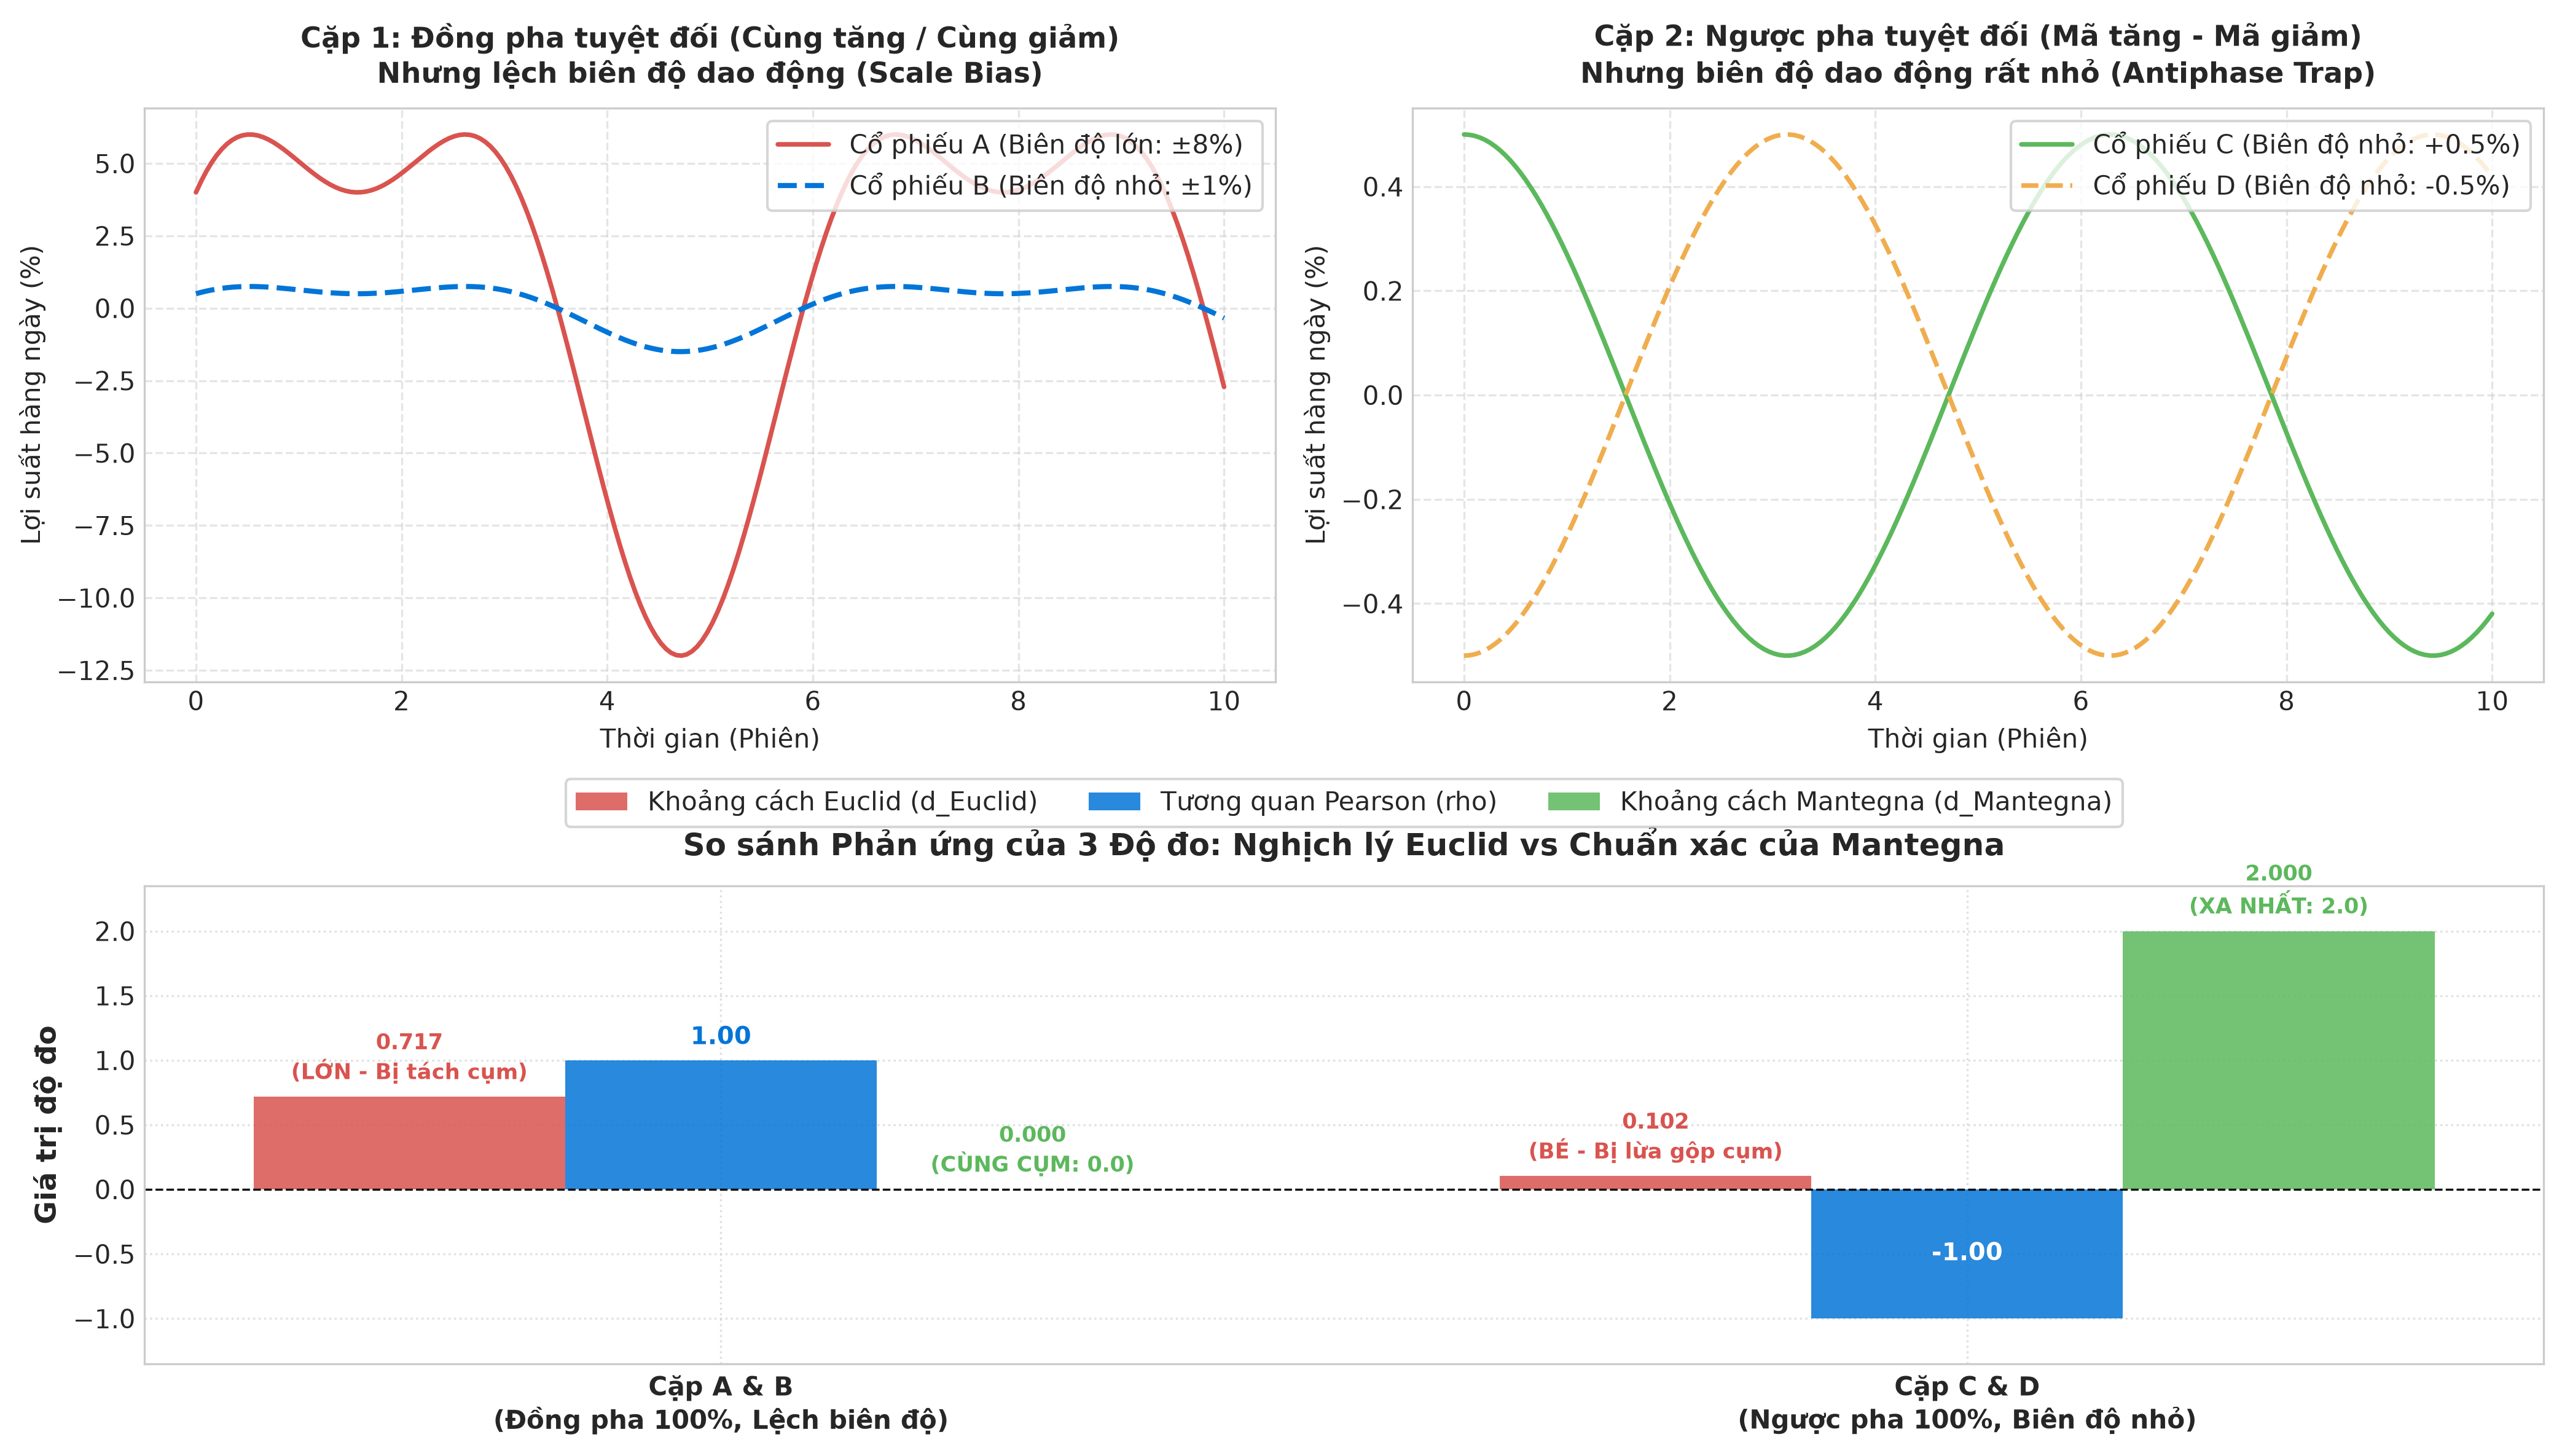
\includegraphics[width=0.92\textwidth]{hinh_euclidean_vs_pearson.png}}
    {\khunghinh{14cm}{7cm}{Hình minh họa Nghịch lý Euclid vs Pearson}}
  \caption{Minh họa nghịch lý khoảng cách Euclid so với tương quan Pearson trên chuỗi tài chính}
  \label{fig:euclid_vs_pearson}
\end{figure}

\subsection{Khoảng cách mêtric Mantegna}
Để triệt tiêu ảnh hưởng của biên độ giá và tập trung đo lường độ đồng biến động pha, hệ số tương quan tuyến tính Pearson được sử dụng:
\begin{equation}
  \rho_{ij} = \frac{\sum_{t=1}^T (r_{i, t} - \bar{r}_i)(r_{j, t} - \bar{r}_j)}{\sqrt{\sum_{t=1}^T (r_{i, t} - \bar{r}_i)^2 \sum_{t=1}^T (r_{j, t} - \bar{r}_j)^2}} \in [-1, 1]
\end{equation}
Mặc dù $\rho_{ij}$ phản ánh chính xác tương quan tuyến tính, nó là một độ đo tương đồng (similarity measure) chứ không phải là một khoảng cách mêtric vì: $\rho_{ii} = 1 \ne 0$, $\rho_{ij}$ có thể mang giá trị âm, và nếu lấy hiệu số $1 - \rho_{ij}$ thì đại lượng này vi phạm bất đẳng thức tam giác. Khi áp dụng các thuật toán phân cụm phân cấp trên độ đo phi mêtric, cây Dendrogram sẽ xảy ra hiện tượng đảo nhánh (tree inversion), làm sai lệch toàn bộ cấu trúc phân cấp.

Nhà vật lý thống kê Rosario N. Mantegna \cite{mantegna1999} đã đề xuất phép biến đổi chuẩn hóa:
\begin{equation}
  d(i, j) = \sqrt{2(1 - \rho_{ij})}
  \label{eq:mantegna}
\end{equation}
Về mặt hình học vi phân, nếu chuẩn hóa các vector lợi suất $r_i$ về giá trị kỳ vọng bằng 0 và phương sai bằng 1 ($z_i = (r_i - \bar{r}_i)/\sigma_i$), thì vector $z_i/\sqrt{T}$ là một điểm nằm trên mặt cầu đơn vị trong không gian $\mathbb{R}^T$. Khi đó, khoảng cách Euclid giữa hai điểm trên mặt cầu đơn vị chính là:
\begin{equation}
  \| z_i^* - z_j^* \|_2^2 = \|z_i^*\|^2 + \|z_j^*\|^2 - 2 \langle z_i^*, z_j^* \rangle = 1 + 1 - 2\rho_{ij} = 2(1 - \rho_{ij})
\end{equation}
Do đó, $d(i, j) = \sqrt{2(1 - \rho_{ij})}$ là khoảng cách Euclid chuẩn tắc trên mặt cầu đơn vị, đảm bảo thỏa mãn đầy đủ 4 tiên đề của một không gian mêtric:
\begin{enumerate}
  \item \textit{Tính không âm:} $d(i, j) \ge 0, \ \forall i, j$.
  \item \textit{Tính đồng nhất:} $d(i, j) = 0 \iff \rho_{ij} = 1$ (hai cổ phiếu biến động giống hệt nhau).
  \item \textit{Tính đối xứng:} $d(i, j) = d(j, i), \ \forall i, j$.
  \item \textit{Bất đẳng thức tam giác:} $d(i, j) \le d(i, k) + d(k, j), \ \forall i, j, k$.
\end{enumerate}

Khoảng cách Mantegna $d(i, j) \in [0, 2]$ có các mốc giá trị thực tiễn rất rõ ràng:
\begin{itemize}
  \item $\rho = 1 \implies d = 0$: Hai cổ phiếu hoàn toàn đồng pha, gom chung cụm.
  \item $\rho = 0 \implies d = \sqrt{2} \approx 1.414$: Hai cổ phiếu độc lập thống kê, lý tưởng cho việc đa dạng hóa danh mục.
  \item $\rho = -1 \implies d = 2.0$: Hai cổ phiếu biến động ngược pha hoàn toàn, tối ưu cho chiến lược phòng hộ rủi ro (Hedging).
\end{itemize}

\begin{figure}[H]
  \centering
  \IfFileExists{images/hinh_mantegna_metric.png}
    {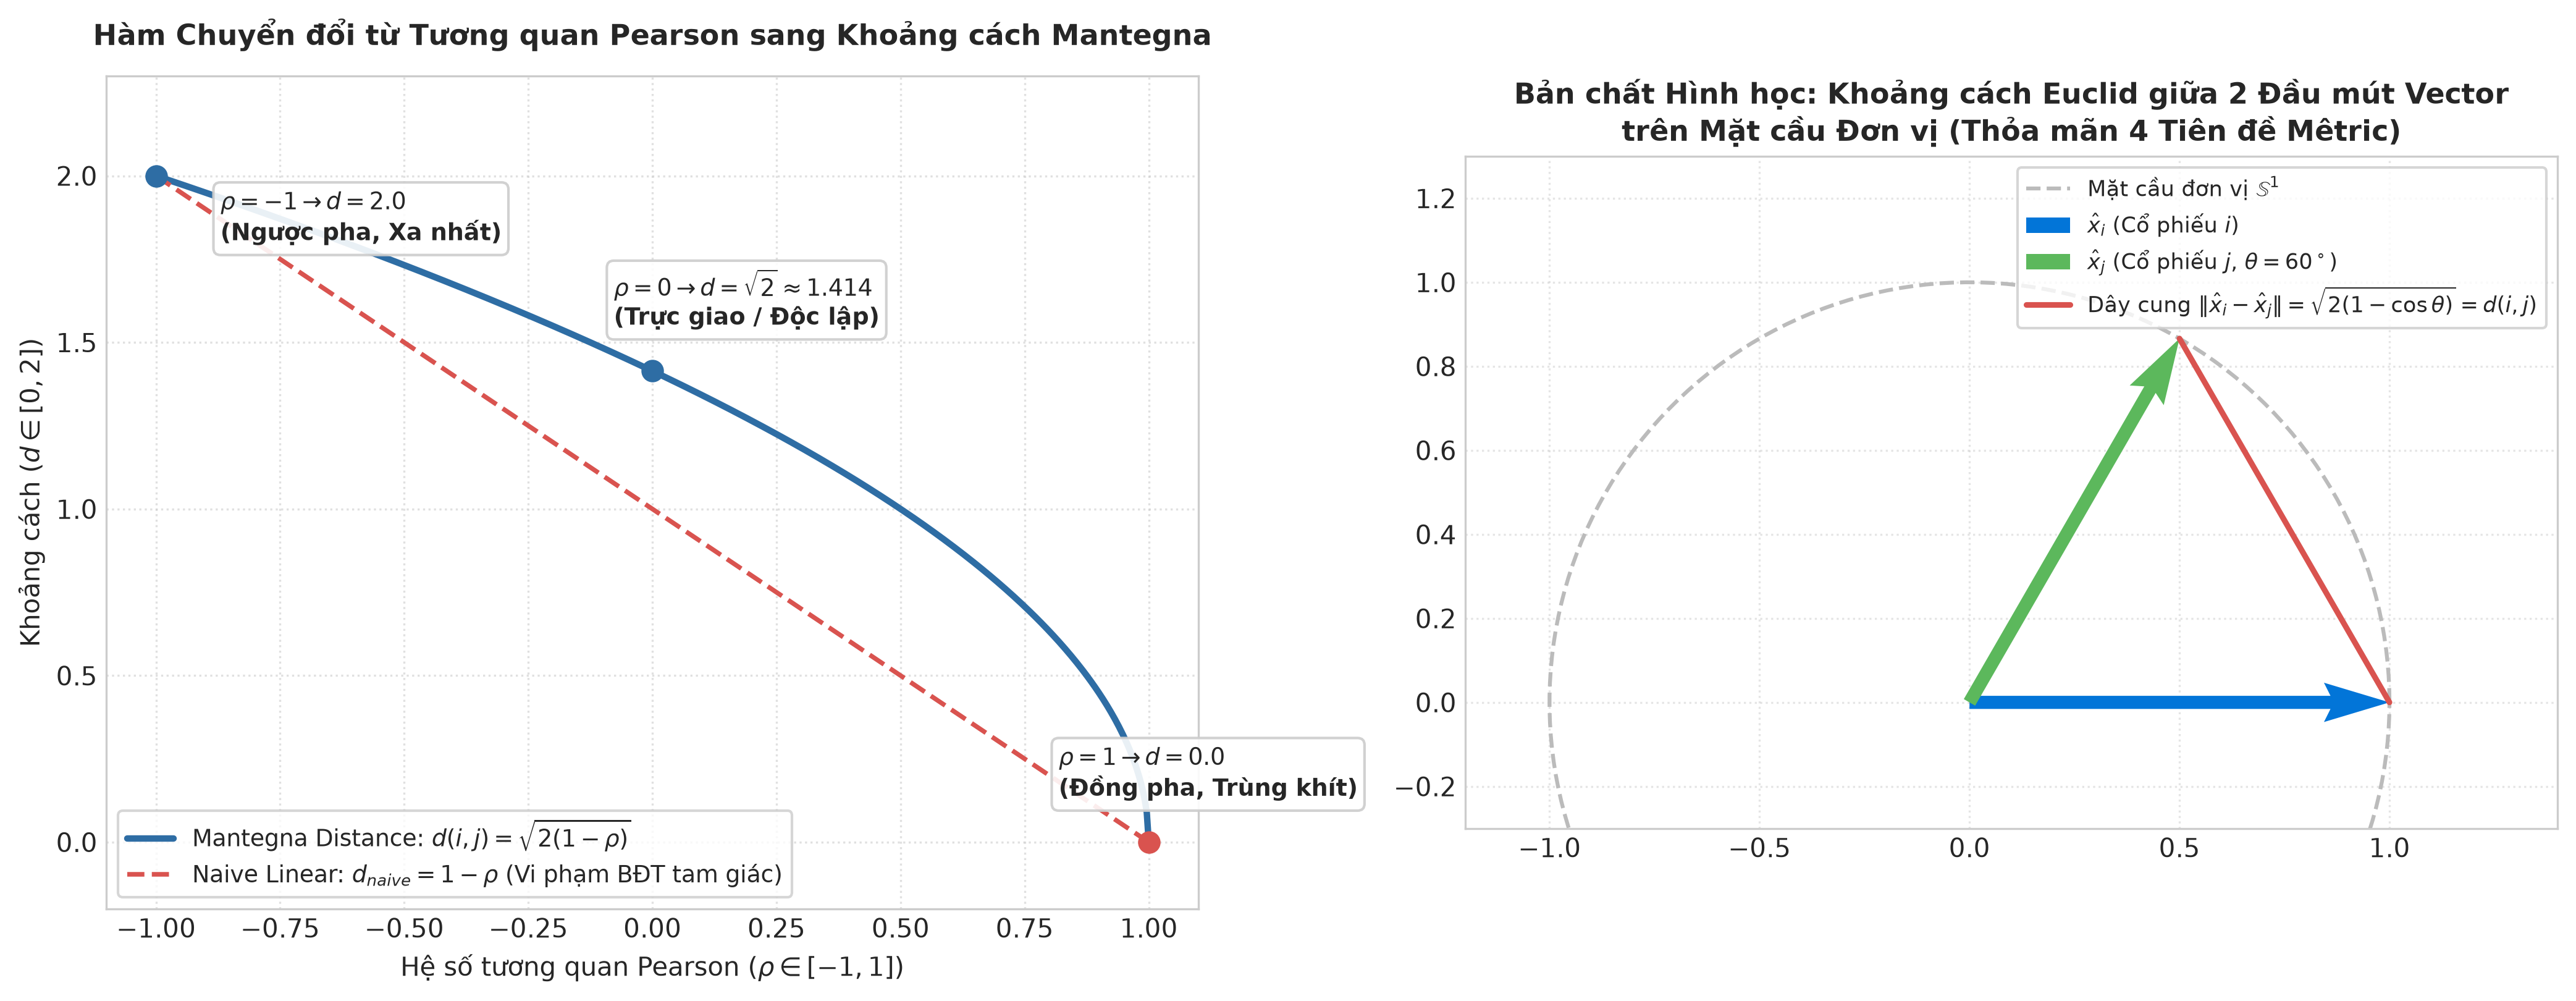
\includegraphics[width=0.92\textwidth]{hinh_mantegna_metric.png}}
    {\khunghinh{14cm}{7cm}{Hình minh họa Phép biến đổi Mantegna}}
  \caption{Phép biến đổi Mantegna từ hệ số tương quan $\rho$ sang khoảng cách mêtric $d$}
  \label{fig:mantegna_metric}
\end{figure}

\section{Lý giải phương pháp phân chia dữ liệu và chỉ số đánh giá}

\subsection{Chiến lược phân chia Hold-out theo thời gian (Chronological Split)}
Trong học máy thông thường, phương pháp kiểm định chéo $K$-Fold ngẫu nhiên (Random $K$-Fold Cross Validation) được áp dụng rộng rãi. Tuy nhiên, đối với dữ liệu tài chính dạng chuỗi thời gian, áp dụng $K$-Fold ngẫu nhiên là một sai lầm nghiêm trọng vì:
\begin{enumerate}
  \item \textit{Vi phạm tính nhân quả thời gian (Look-ahead bias):} Việc xáo trộn ngẫu nhiên khiến các điểm dữ liệu trong tương lai bị rò rỉ vào tập huấn luyện để dự đoán các quan sát trong quá khứ.
  \item \textit{Tự tương quan chuỗi (Serial Correlation):} Lợi suất tài chính có tính chất tụ cụm biến động (Volatility Clustering); dữ liệu ngày hôm trước có tương quan thông tin mạnh với ngày hôm sau. Xáo trộn ngẫu nhiên làm thổi phồng hiệu năng mô hình một cách giả tạo.
\end{enumerate}

Theo Marcos López de Prado (2018), phương pháp duy nhất đúng đắn là phân chia theo trục thời gian tuyến tính (Chronological In-Sample vs Out-of-Sample Split). Trong đề tài này, đơn vị mẫu là $N = 98$ cổ phiếu; đặc trưng của mỗi cổ phiếu là chuỗi thời gian 1.186 phiên. Do đó, việc phân chia phải thực hiện trên trục thời gian (phiên giao dịch) thay vì chia trên danh sách cổ phiếu (nếu bỏ bớt cổ phiếu thì không thể phân cụm hay lập danh mục cho các cổ phiếu đó).

\subsection{Cơ sở Lý thuyết Ma trận Ngẫu nhiên (Random Matrix Theory -- RMT)}
Để đảm bảo ma trận tương quan trên tập huấn luyện không bị nhiễu ngẫu nhiên chi phối, số lượng phiên giao dịch $T$ trong tập Train phải thỏa mãn tiêu chuẩn của Lý thuyết Ma trận Ngẫu nhiên (Bouchaud \& Potters, 2000; Laloux et al., 1999). Theo định lý Marchenko-Pastur, khi tỷ số chất lượng dữ liệu:
\begin{equation}
  Q = \frac{T}{N}
\end{equation}
tiệm cận về 1 hoặc nhỏ hơn 1, các trị riêng của ma trận tương quan mẫu sẽ bị bao phủ hoàn toàn bởi dải nhiễu ngẫu nhiên $[\lambda_-, \lambda_+]$:
\begin{equation}
  \lambda_{\pm} = \left(1 \pm \sqrt{\frac{1}{Q}}\right)^2
\end{equation}
Để cấu trúc tương quan tài chính bộc lộ rõ nét và các trị riêng mang thông tin thực sự tách biệt khỏi dải nhiễu, tỷ số $Q$ bắt buộc phải lớn hơn 3 đến 5. Với $N = 98$ cổ phiếu, nhóm thiết kế tập Train gồm $T_{\text{train}} = 739$ phiên giao dịch (3 năm tròn 2022--2024), đạt tỷ số:
\begin{equation}
  Q_{\text{train}} = \frac{739}{98} \approx 7.54 \gg 1
\end{equation}
Tỷ số này đảm bảo ma trận tương quan In-Sample có độ tin cậy thống kê cao nhất, lọc sạch nhiễu trắng trước khi tiến hành phân cụm.

% =====================================================================
%  CHƯƠNG 2
% =====================================================================
\chapter{Thu thập và khảo sát thống kê dữ liệu}
\label{chap:thuthapvakhaosat}

\section{Nguồn thu thập và điều kiện sử dụng dữ liệu}
Dữ liệu sử dụng trong nghiên cứu được thu thập từ nguồn dữ liệu thị trường chứng khoán Việt Nam thông qua giao thức API của thư viện \texttt{vnstock} (kết nối máy chủ dữ liệu Công ty Chứng khoán Kỹ thương -- TCBS) và nguồn kiểm chứng phụ trợ Yahoo Finance. 

Điều kiện sử dụng dữ liệu tuân thủ nghiêm ngặt các quy định về nghiên cứu học thuật và phi thương mại:
\begin{itemize}
  \item Dữ liệu giá giao dịch lịch sử là thông tin công khai trên các sở giao dịch chứng khoán.
  \item Việc trích xuất dữ liệu tự động được thực hiện qua các hàm API có giới hạn tần suất (rate-limiting) để đảm bảo không gây tải cho máy chủ cung cấp dữ liệu.
  \item Toàn bộ dữ liệu thô sau khi tải về được lưu trữ cục bộ dưới định dạng CSV tại thư mục \texttt{data/raw/} với mốc thời gian rõ ràng để đảm bảo tính minh bạch và khả năng tái lập thực nghiệm.
\end{itemize}

\section{Không gian mẫu và từ điển dữ liệu}
Không gian nghiên cứu bao gồm 100 cổ phiếu thành phần rổ chỉ số VN100 trên sàn HOSE giai đoạn từ 01/01/2022 đến 23/10/2026. Danh sách mã và thông tin phân ngành cấp 1 theo chuẩn quốc tế ICB (Industry Classification Benchmark) được lưu trữ tại \texttt{data/metadata/vn100\_symbols.csv}, phân bổ trên 11 nhóm ngành chính: Bất động sản, Ngân hàng, Dịch vụ tài chính (Chứng khoán), Tài nguyên cơ bản (Thép), Hàng tiêu dùng, Bán lẻ, Xây dựng \& Vật liệu, Hóa chất, Tiện ích (Điện, Nước, Khí đốt), Công nghệ thông tin và Viễn thông.

Để mô tả đầy đủ các thuộc tính phân phối và rủi ro của từng cổ phiếu, nhóm xây dựng Từ điển dữ liệu gồm 8 chỉ số tài chính định lượng được tính toán từ chuỗi lợi suất logarit, lưu tại \texttt{data/processed/stock\_financial\_features.csv} và được mô tả chi tiết trong Bảng~\ref{tab:tudien}.

\begin{table}[H]
  \centering
  \caption{Từ điển dữ liệu các đặc trưng tài chính trích chọn từ chuỗi lợi suất}
  \label{tab:tudien}
  \begin{tabularx}{\textwidth}{|>{\centering\arraybackslash}p{1cm}|p{4.3cm}|>{\centering\arraybackslash}p{1.6cm}|X|}
    \hline
    \rowcolor{black!8}\textbf{STT} & \textbf{Tên đặc trưng} & \textbf{Kiểu dữ liệu} & \textbf{Mô tả ý nghĩa tài chính và công thức} \\ \hline
    1 & \textbf{symbol} & String & Mã chứng khoán niêm yết trên sàn HOSE (ví dụ: VCB, FPT, HPG) \\ \hline
    2 & \textbf{mean\_daily\_pct} & Float & Lợi suất trung bình ngày (\%): $\bar{r} = \frac{1}{T}\sum_{t=1}^T r_t \times 100\%$ \\ \hline
    3 & \textbf{annual\_return\_pct} & Float & Lợi suất bình quân hàng năm (\%): $\mu_{ann} = \bar{r} \times 252$ (chuẩn hóa 252 phiên giao dịch/năm) \\ \hline
    4 & \textbf{annual\_volatility\_pct} & Float & Độ biến động (rủi ro) bình quân năm (\%): $\sigma_{ann} = \text{std}(r) \times \sqrt{252} \times 100\%$ \\ \hline
    5 & \textbf{sharpe\_ratio} & Float & Tỷ số Sharpe đo hiệu quả sinh lời trên một đơn vị rủi ro với lãi suất phi rủi ro $r_f = 4.5\%$: $SR = \frac{\mu_{ann} - r_f}{\sigma_{ann}}$ \\ \hline
    6 & \textbf{skewness} & Float & Hệ số độ lệch phân phối lợi suất: đo tính bất đối xứng so với phân phối chuẩn Gauss \\ \hline
    7 & \textbf{excess\_kurtosis} & Float & Hệ số độ nhọn dư: $\text{Kurt} - 3.0$; giá trị $> 0$ phản ánh hiện tượng đuôi béo (Fat-tails) \\ \hline
    8 & \textbf{jb\_pvalue} & Float & $p$-value của kiểm định Jarque-Bera kiểm tra tính phân phối chuẩn của chuỗi lợi suất \\ \hline
  \end{tabularx}
\end{table}

\section{Khảo sát thống kê mô tả chuỗi thời gian giá}
Sau khi làm sạch dữ liệu (loại bỏ 2 mã thiếu và xử lý ngày lễ), không gian mẫu đạt kích thước chuẩn hóa 1.187 phiên giao dịch cho 98 mã cổ phiếu. Hình~\ref{fig:clean_price} minh họa diễn biến chuỗi giá đóng cửa điều chỉnh của 98 cổ phiếu sau khi quy đổi về mốc cơ sở 100 tại phiên giao dịch đầu tiên (04/01/2022).

\begin{figure}[H]
  \centering
  \IfFileExists{images/hinh_clean_price_series.png}
    {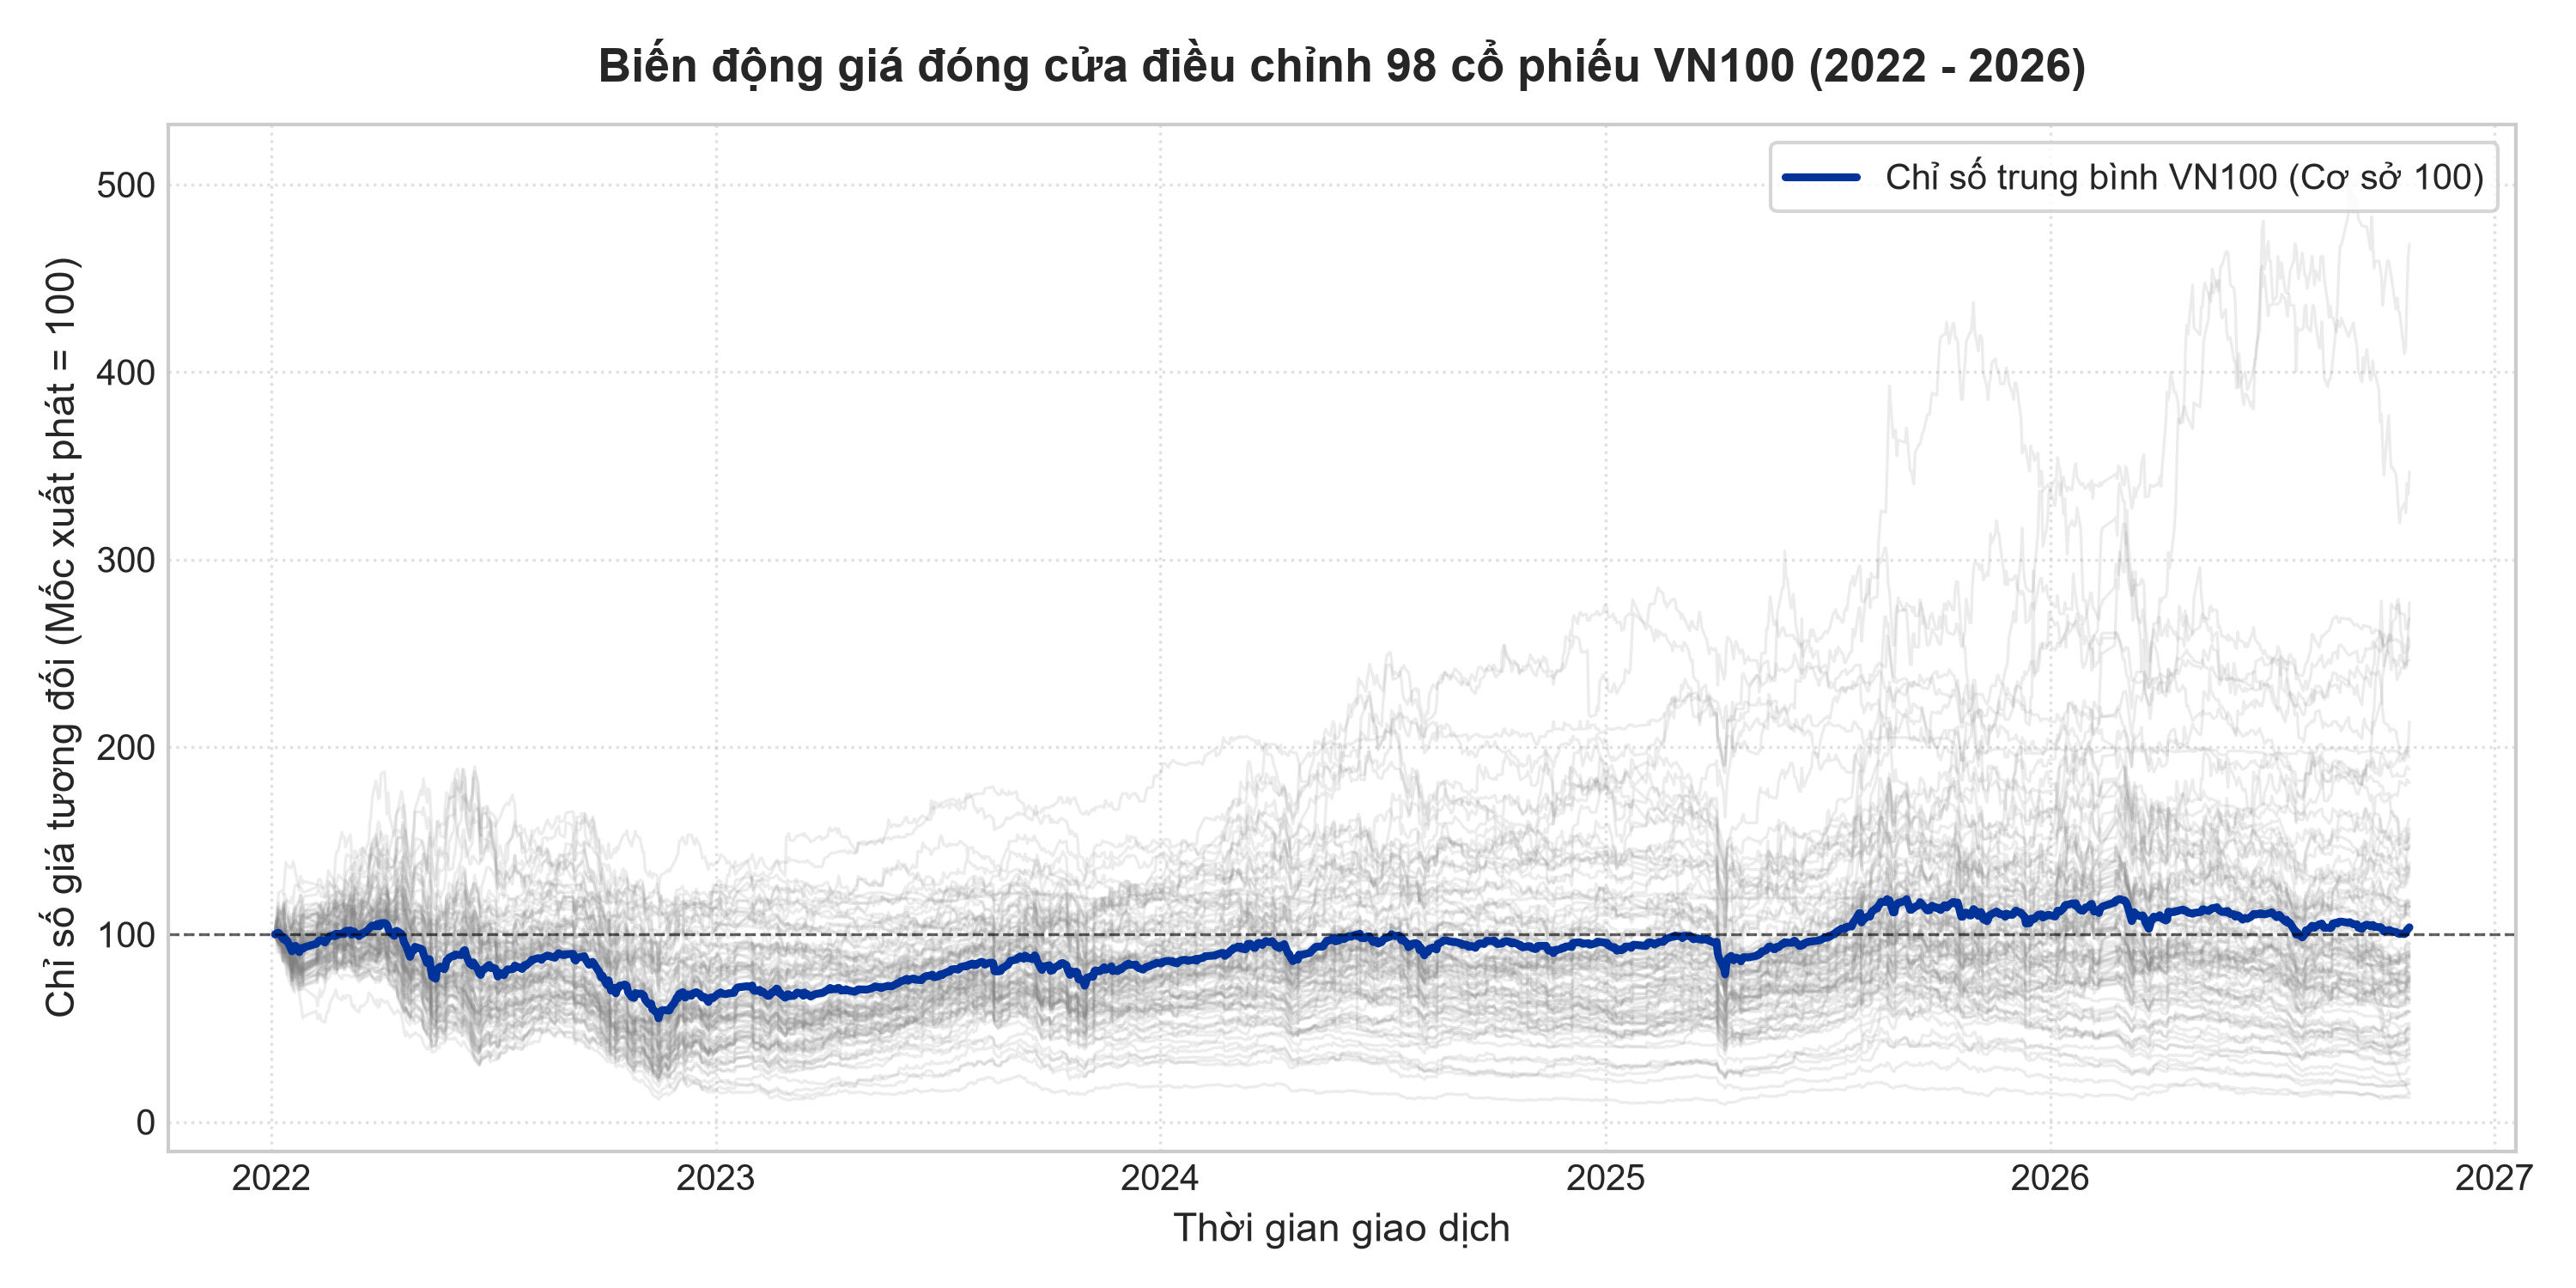
\includegraphics[width=0.95\textwidth]{hinh_clean_price_series.png}}
    {\khunghinh{14cm}{7cm}{Biểu đồ đường giá sau khi làm sạch}}
  \caption{Diễn biến giá đóng cửa điều chỉnh chuẩn hóa (cơ sở 100) của 98 cổ phiếu VN100}
  \label{fig:clean_price}
\end{figure}

\textbf{Nhận xét từ biểu đồ giá:}
\begin{itemize}
  \item \textit{Pha giảm mạnh năm 2022:} Thị trường chịu áp lực bán tháo diện rộng, chỉ số trung bình rổ VN100 sụt giảm từ mốc 100 điểm xuống đáy khoảng 55 điểm (mức giảm gần 45\%), tạo ra mức độ tương quan sụt giảm rất cao giữa các cổ phiếu.
  \item \textit{Pha phục hồi phân hóa 2023--2024:} Thị trường tạo đáy và bước vào nhịp phục hồi tái tích lũy; tuy nhiên, mức độ phục hồi có sự phân hóa sâu sắc: một số cổ phiếu nhóm Công nghệ (FPT) và Ngân hàng chất lượng cao bứt phá vượt đỉnh lịch sử, trong khi nhiều cổ phiếu Bất động sản và Xây dựng vẫn dao động quanh vùng đáy.
  \item \textit{Pha đi ngang tích lũy 2025--2026:} Thị trường dao động trong biên độ hẹp quanh vùng 75--85 điểm cơ sở, phản ánh đặc tính phân hóa theo kết quả hoạt động kinh doanh riêng lẻ của từng doanh nghiệp.
\end{itemize}

\section{Phân tích phân bố lợi suất và kiểm định hiện tượng đuôi béo (Fat-tails)}
Lợi suất logarit hàng ngày của cổ phiếu $i$ tại phiên $t$ được xác định theo công thức:
\begin{equation}
  r_{i, t} = \ln(P_{i, t}) - \ln(P_{i, t-1})
\end{equation}
Toàn bộ ma trận lợi suất gồm $1.186 \text{ phiên} \times 98 \text{ mã} = 116.228$ quan sát được khảo sát phân bố thống kê. Kết quả phân tích phân bố và biểu đồ Q-Q Plot kiểm định phân phối chuẩn được trình bày trong Hình~\ref{fig:returns_qq}.

\begin{figure}[H]
  \centering
  \IfFileExists{images/hinh_returns_distribution_qq.png}
    {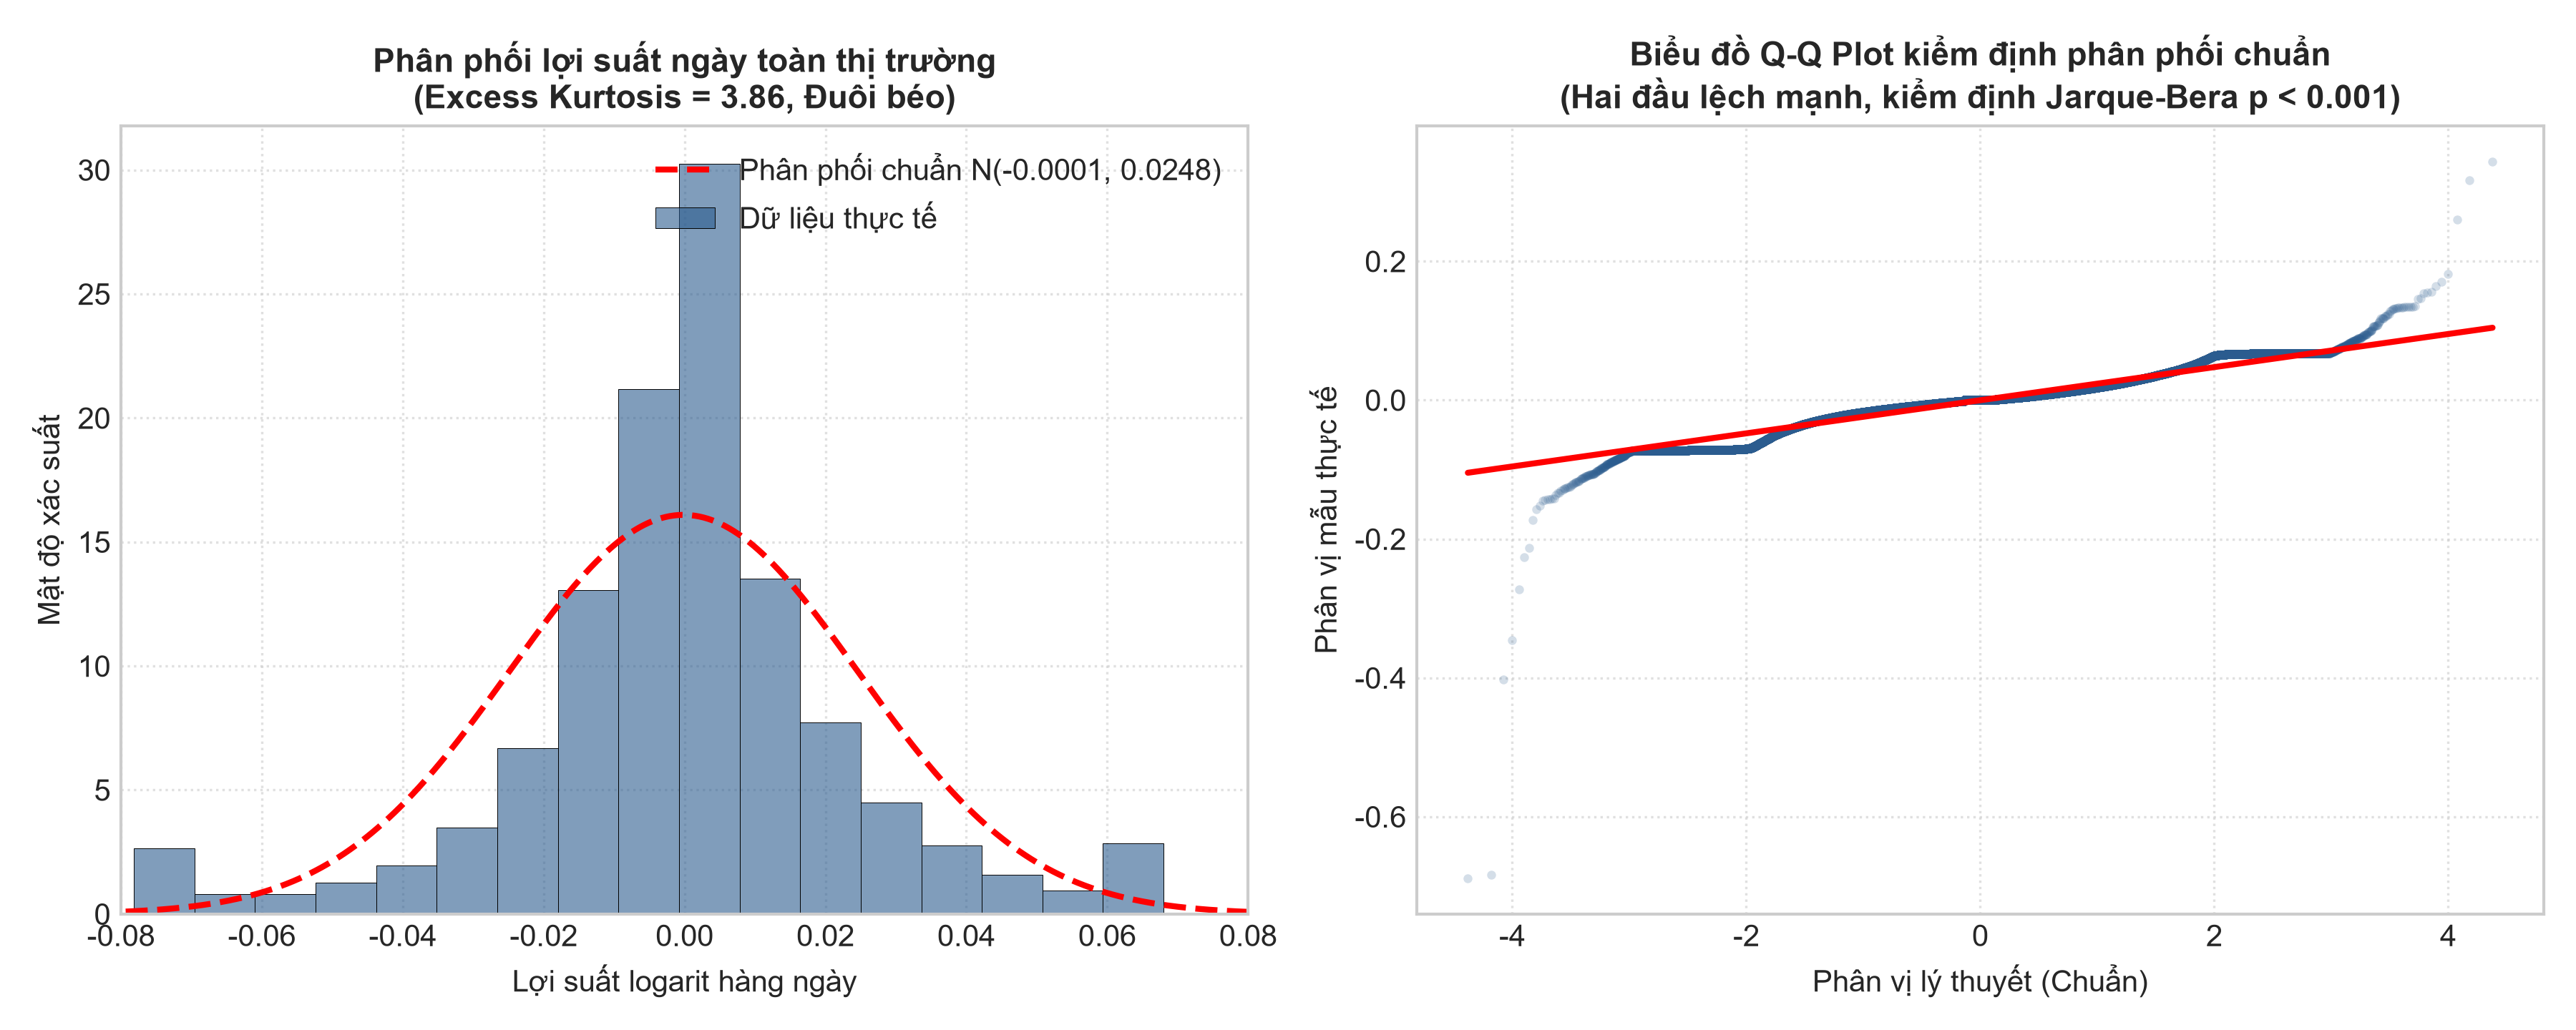
\includegraphics[width=0.95\textwidth]{hinh_returns_distribution_qq.png}}
    {\khunghinh{14cm}{6cm}{Phân phối lợi suất và Q-Q Plot}}
  \caption{Phân phối tần suất lợi suất logarit và biểu đồ Q-Q Plot toàn thị trường VN100}
  \label{fig:returns_qq}
\end{figure}

\textbf{Kết quả định lượng và nhận xét thống kê:}
\begin{itemize}
  \item \textit{Lợi suất trung bình năm:} Toàn thị trường ghi nhận mức lợi suất bình quân $\bar{\mu}_{ann} = -3.65\%/\text{năm}$, do giai đoạn 2022 có nhịp điều chỉnh giảm sâu.
  \item \textit{Độ biến động trung bình năm:} Mức biến động bình quân $\bar{\sigma}_{ann} = 38.54\%/\text{năm}$, phản ánh tính biến động mạnh đặc thù của thị trường chứng khoán mới nổi Việt Nam.
  \item \textit{Hệ số độ lệch (Skewness):} Đạt giá trị âm nhẹ ($\text{Skew} = -0.18$), phản ánh đặc trưng bất đối xứng: thị trường có xu hướng giảm nhanh, mạnh và dốc hơn so với các nhịp tăng từ tốn.
  \item \textit{Hệ số độ nhọn dư (Excess Kurtosis):} Đạt mức trung bình $3.86 > 0$ (vượt trội hoàn toàn so với mức 0 của phân phối chuẩn Gauss). Đỉnh phân phối nhọn hơn và hai đuôi dày hơn đáng kể.
  \item \textit{Kiểm định Jarque-Bera:} 98/98 mã cổ phiếu đều có giá trị kiểm định với mức ý nghĩa $p$-value $< 0.001$, bác bỏ hoàn toàn giả thuyết phân phối chuẩn.
  \item \textit{Ý nghĩa đối với mô hình học máy:} Thị trường thực tế tồn tại hiện tượng \textbf{đuôi béo (Fat-tails)} rõ rệt; xác suất xảy ra các phiên biến động kịch trần hoặc kịch sàn ($\pm 7\%$) cao gấp hàng chục lần so với giả định của phân phối chuẩn Gauss. Điều này khẳng định sự cần thiết của việc sử dụng các độ đo khoảng cách phi tuyến và tương quan hạng thay vì các phương pháp hồi quy tham số truyền thống.
\end{itemize}

\section{Khảo sát không gian Lợi suất -- Rủi ro (Risk-Return Trade-off)}
Hình~\ref{fig:risk_return} biểu diễn vị trí của 98 cổ phiếu trong không gian hai chiều giữa Độ biến động hàng năm (Rủi ro $\sigma_{ann}$) và Lợi suất hàng năm ($\mu_{ann}$), có tô màu phân loại theo 11 nhóm ngành ICB.

\begin{figure}[H]
  \centering
  \IfFileExists{images/hinh_risk_return_scatter.png}
    {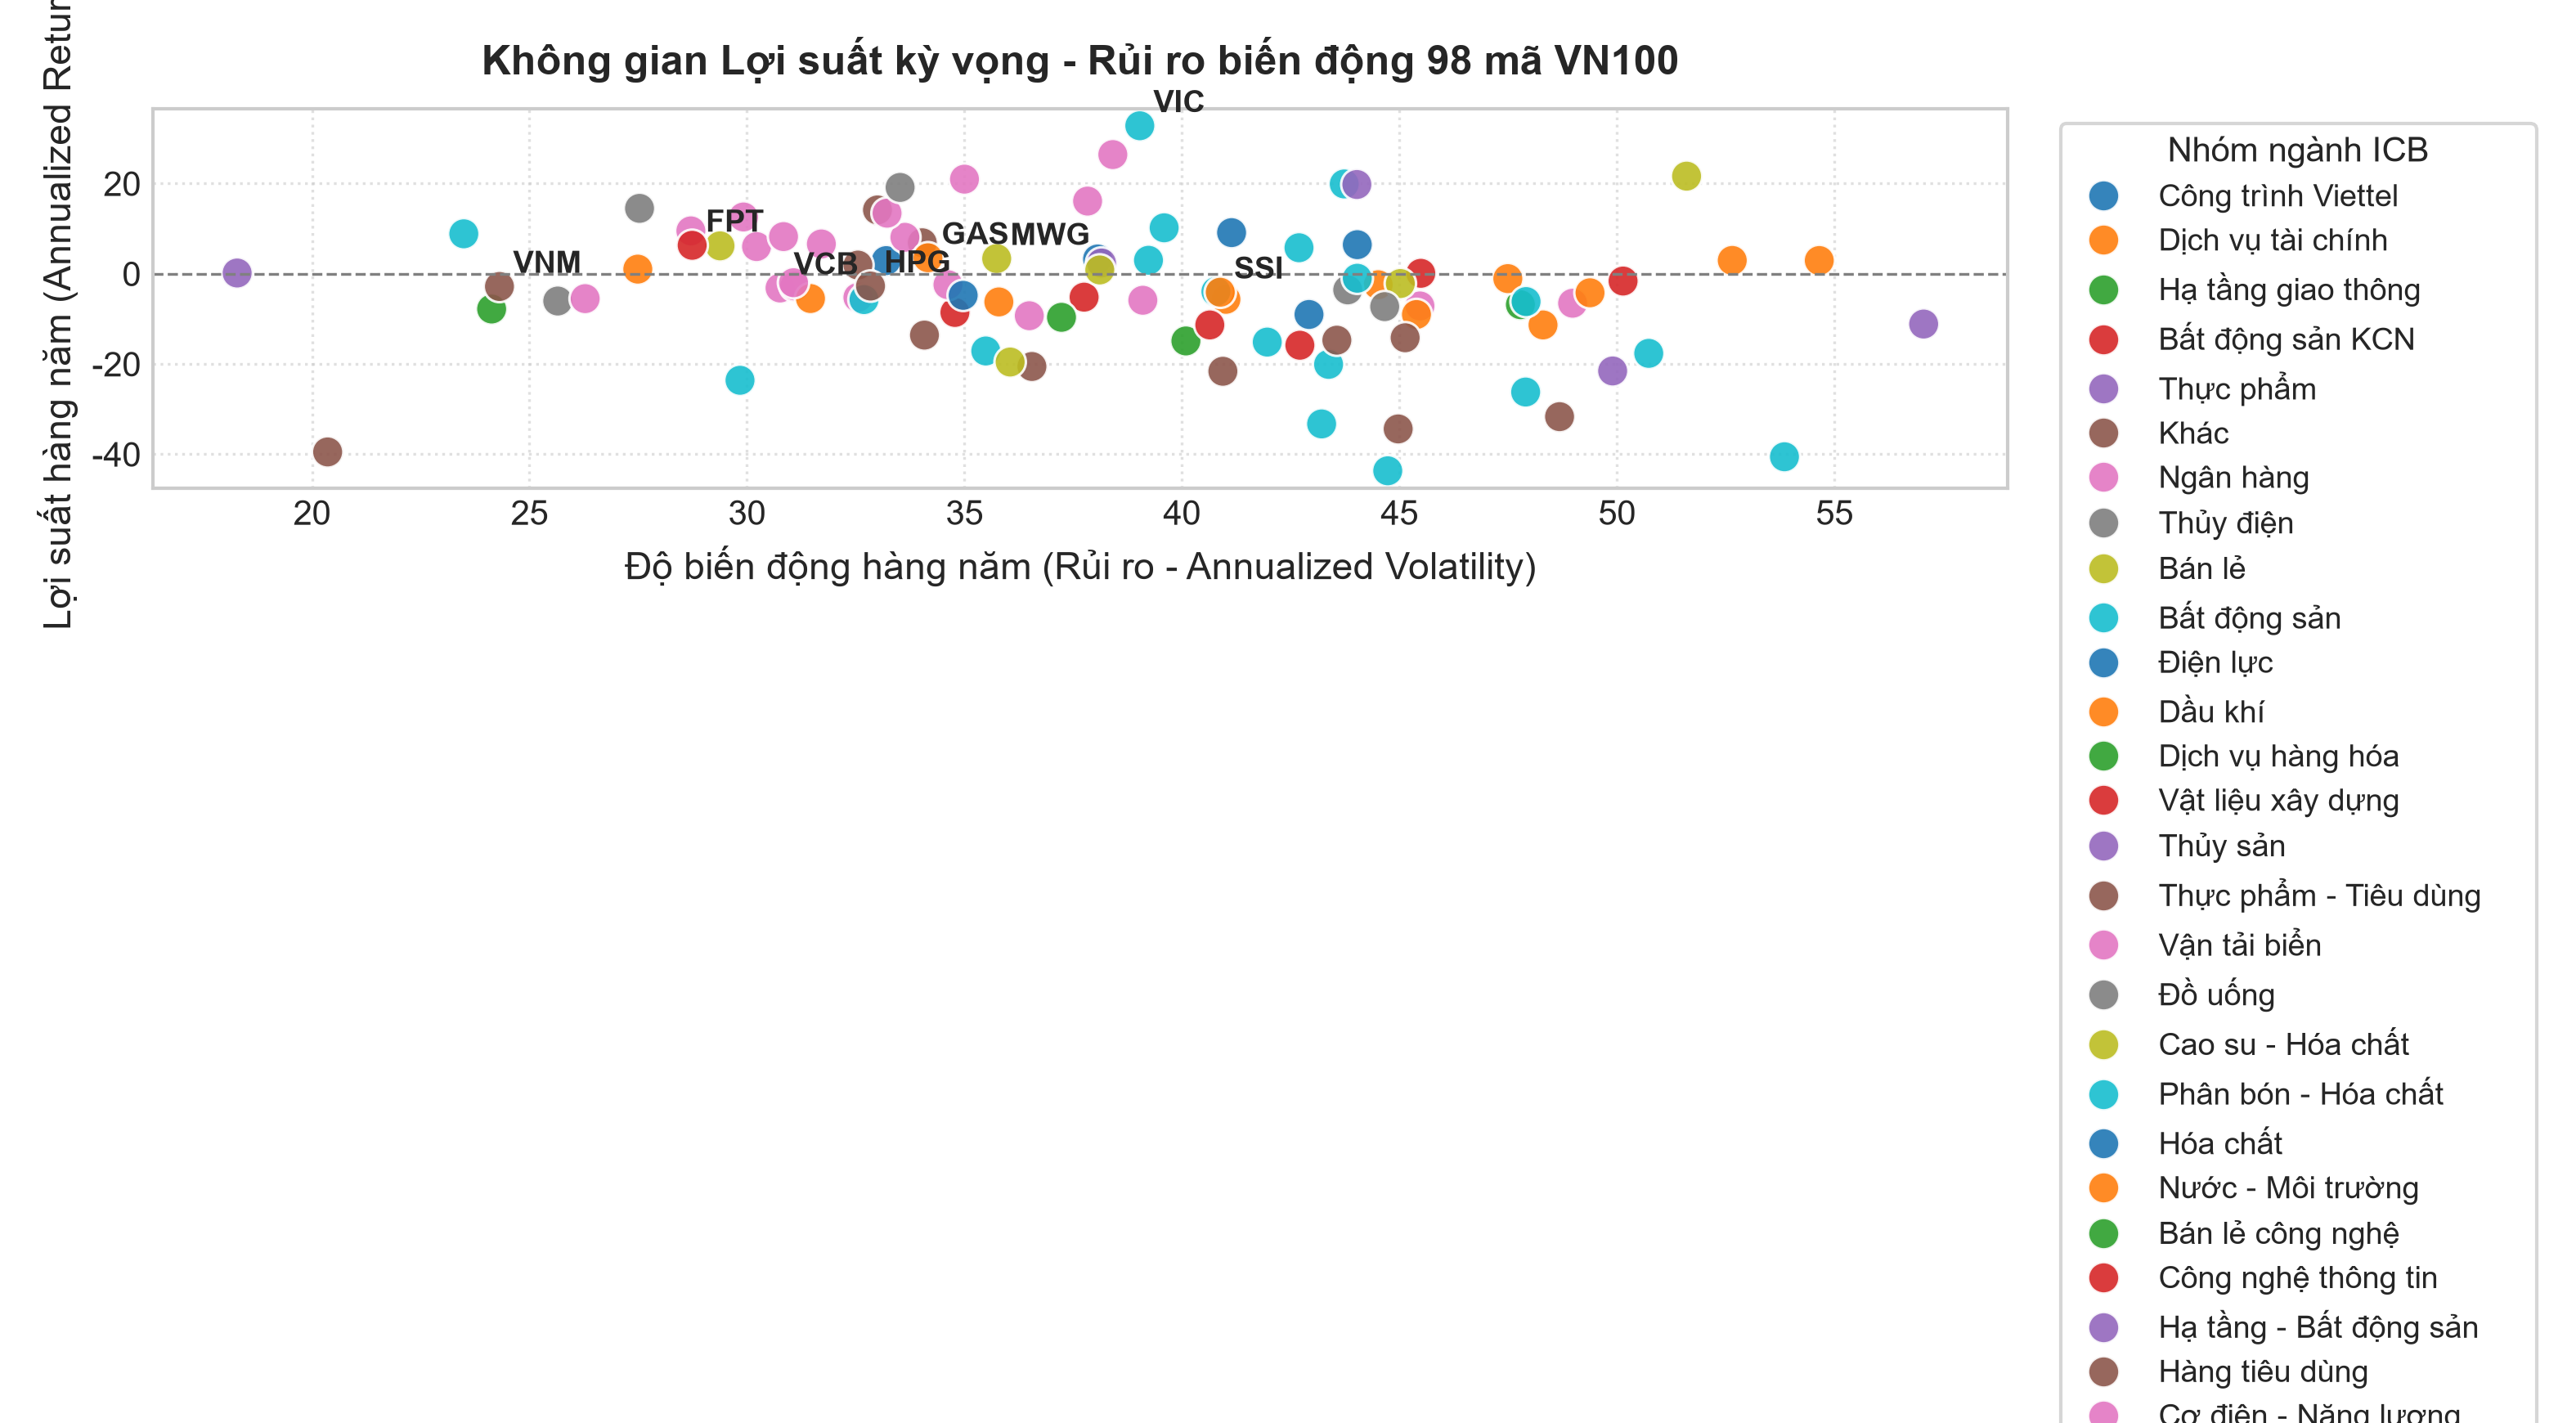
\includegraphics[width=0.95\textwidth]{hinh_risk_return_scatter.png}}
    {\khunghinh{14cm}{7cm}{Biểu đồ phân tán Lợi suất - Rủi ro theo ICB}}
  \caption{Không gian Lợi suất kỳ vọng -- Rủi ro biến động của 98 cổ phiếu theo nhóm ngành ICB}
  \label{fig:risk_return}
\end{figure}

\textbf{Nhận xét phân tích cấu trúc rủi ro -- lợi suất:}
\begin{enumerate}
  \item \textit{Khối Ngân hàng (Banking):} Tập trung ở vùng biến động trung bình thấp ($\sigma \in [25\%, 35\%]$) và có tỷ suất sinh lời ổn định (đại diện tiêu biểu: VCB, ACB, BID, MBB). Tỷ số Sharpe của nhóm này thuộc nhóm cao nhất thị trường.
  \item \textit{Khối Bất động sản (Real Estate):} Nằm lệch hẳn về phía rủi ro cực cao ($\sigma \in [45\%, 65\%]$) và có mức lợi suất âm sâu trong giai đoạn 2022--2026 (tiêu biểu: NVL, DIG, PDR, DXG).
  \item \textit{Cổ phiếu Công nghệ vượt trội:} Mã FPT nằm ở góc phần tư lý tưởng (lợi suất hàng năm $> 25\%$ với độ biến động chỉ xấp xỉ $28\%$), đạt tỷ số Sharpe cao nhất rổ VN100 ($SR > 0.85$).
  \item \textit{Khối Tiện ích \& Năng lượng (Utilities):} Các mã như GAS, POW có độ biến động rất thấp, dao động độc lập với chu kỳ thị trường chung.
\end{enumerate}

\section{Phân tích ma trận tương quan và quan hệ giữa các cổ phiếu}
Ma trận tương quan Pearson kích thước $98 \times 98$ được tính toán trên toàn bộ 1.186 phiên giao dịch sạch. Để chuẩn bị dữ liệu huấn luyện độc lập cho mô hình, nhóm tính toán ma trận tương quan riêng biệt trên tập Train ($739$ phiên) như hiển thị trong Hình~\ref{fig:train_corr_heatmap}.

\begin{figure}[H]
  \centering
  \IfFileExists{images/hinh_train_correlation_heatmap.png}
    {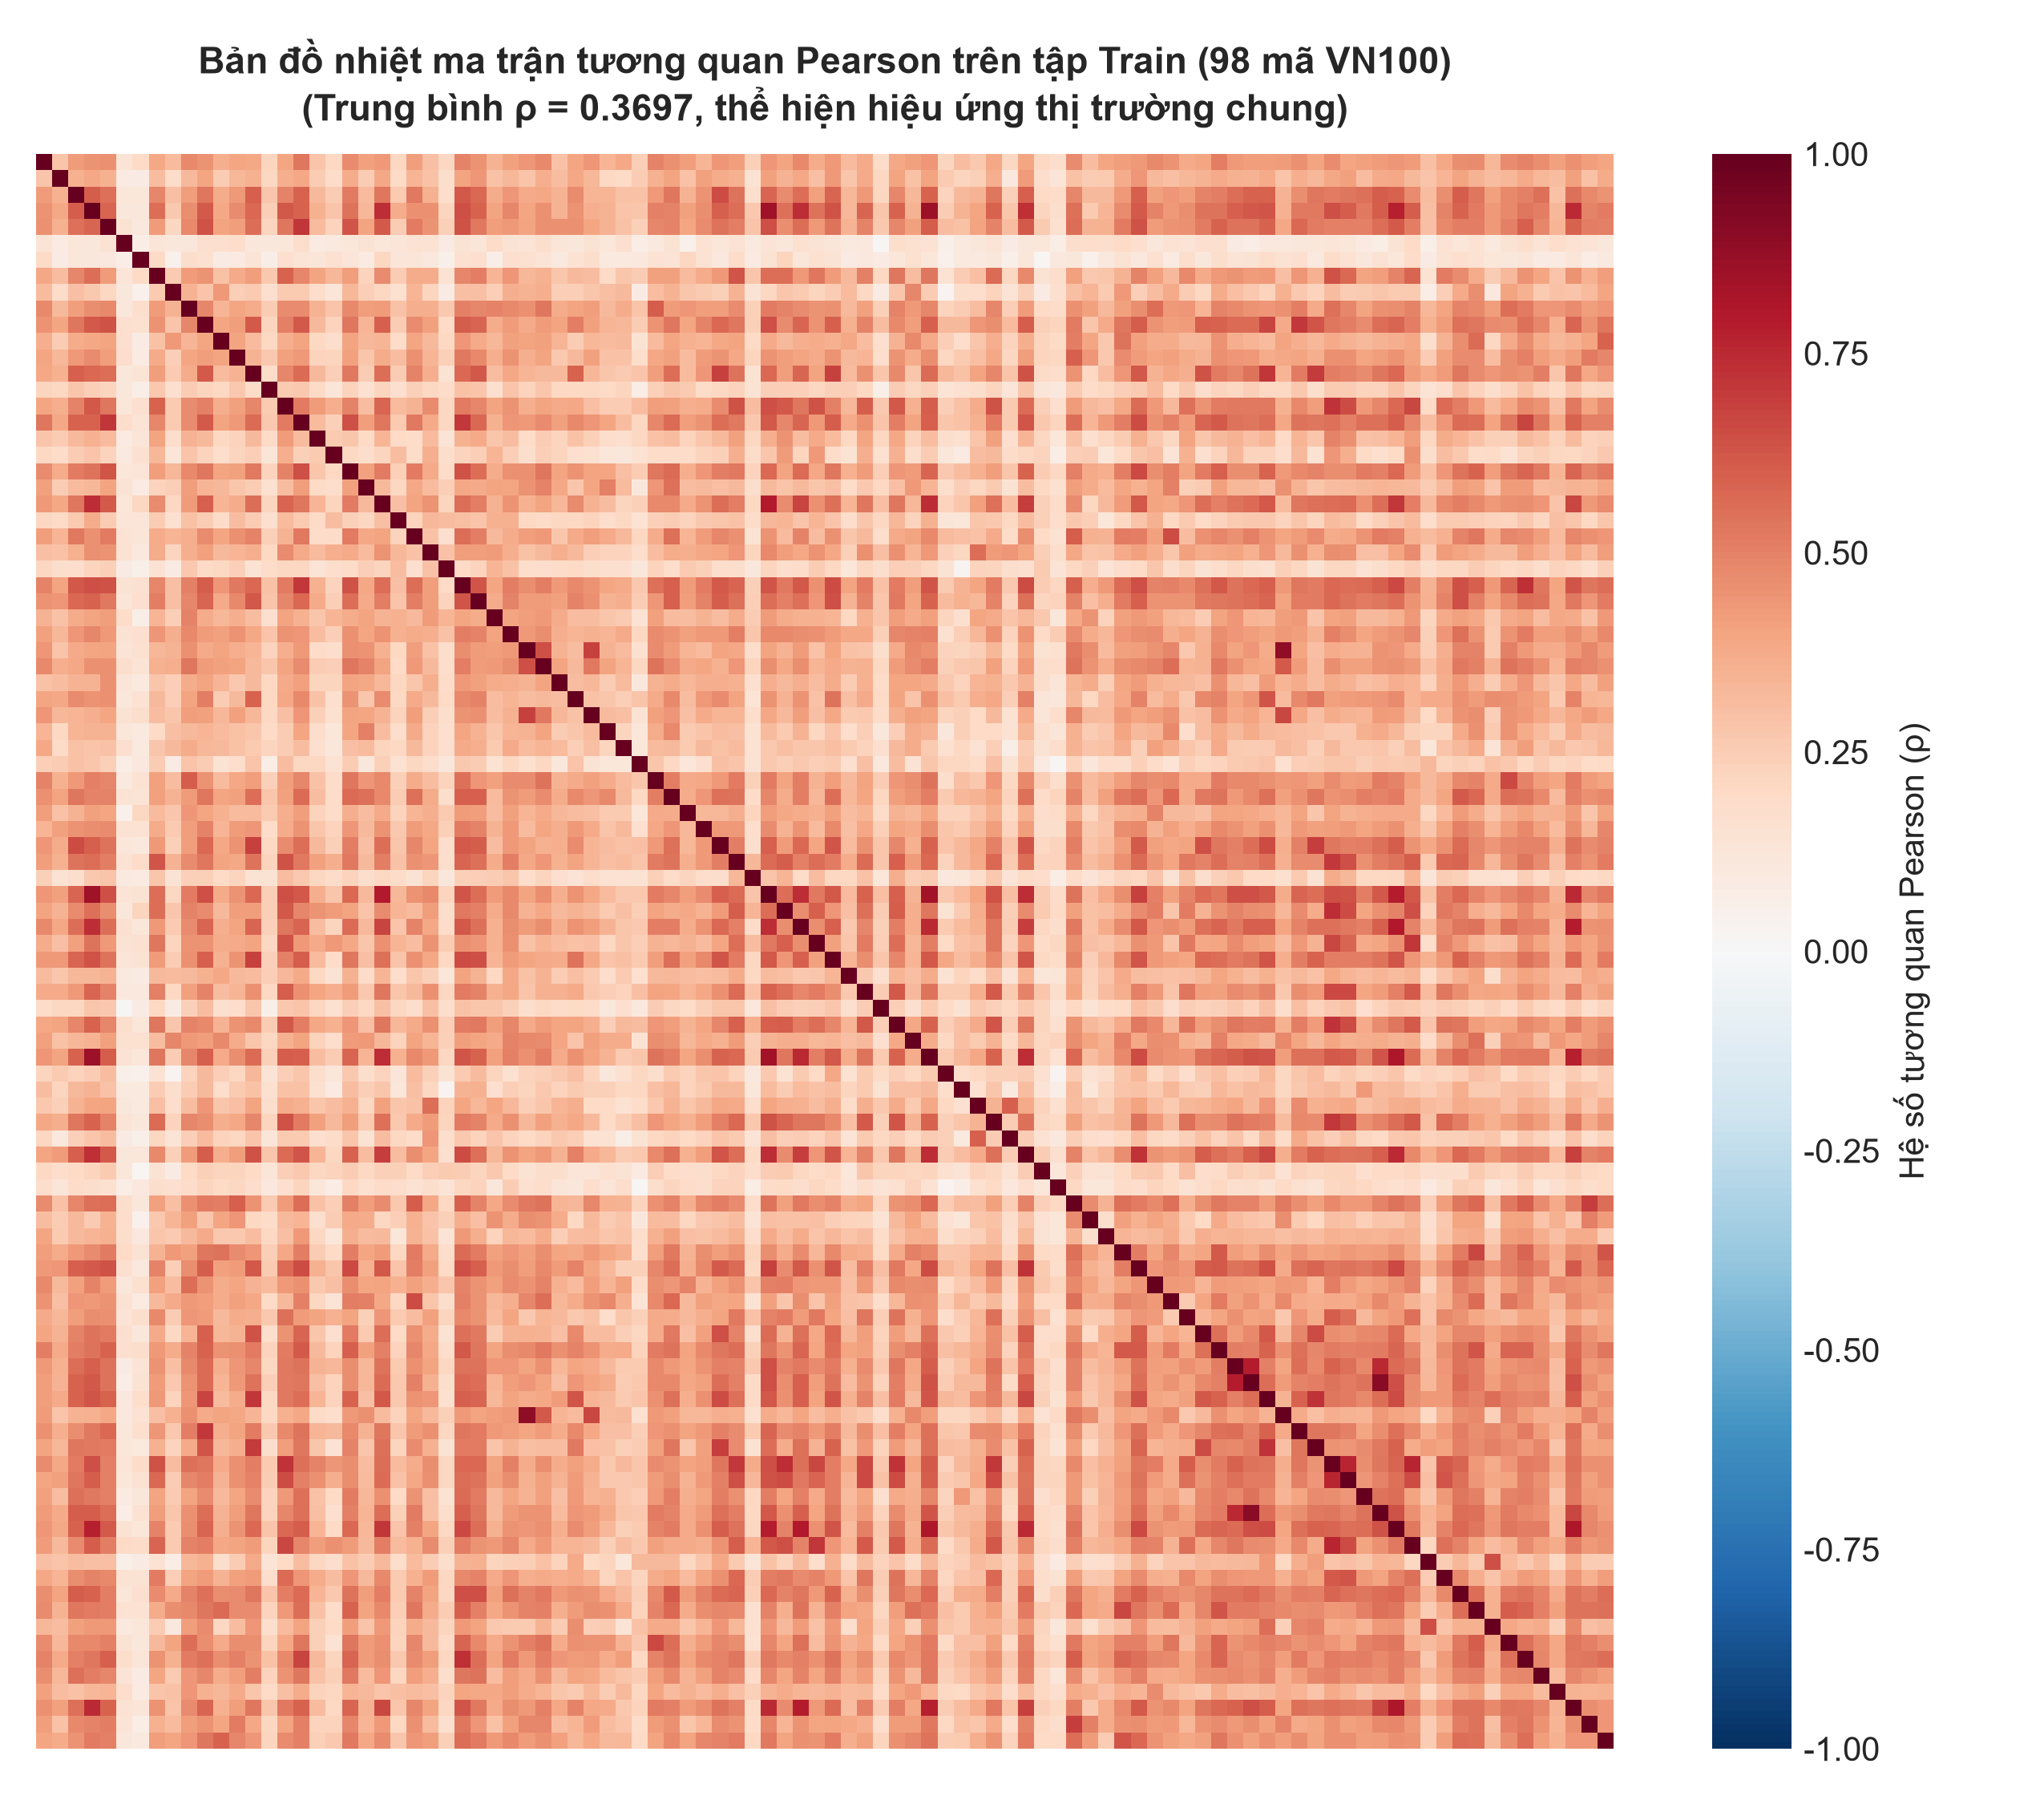
\includegraphics[width=0.82\textwidth]{hinh_train_correlation_heatmap.png}}
    {\khunghinh{12cm}{10cm}{Bản đồ nhiệt tương quan Pearson tập Train}}
  \caption{Bản đồ nhiệt ma trận tương quan Pearson tập Train ($98 \times 98$ cổ phiếu)}
  \label{fig:train_corr_heatmap}
\end{figure}

Từ việc phân tích cấu trúc ma trận tương quan, nhóm rút ra \textbf{4 nhận xét cốt lõi} có ý nghĩa quyết định cho việc thiết kế mô hình phân cụm:
\begin{enumerate}
  \item \textit{Nhận xét 1 -- Hiệu ứng thị trường chung (Market Mode):} Hệ số tương quan Pearson bình quân giữa tất cả các cặp cổ phiếu trên tập Train mang giá trị dương khá cao ($\bar{\rho}_{\text{train}} = 0.3697 > 0$; toàn kỳ $\bar{\rho} = 0.3168$). Không có cặp cổ phiếu nào có tương quan âm sâu ($\rho < -0.15$). Điều này phản ánh tâm lý thị trường chứng khoán Việt Nam bị chi phối mạnh bởi yếu tố thị trường chung (chỉ số VN-Index); khi thị trường hoảng loạn hoặc hưng phấn, phần lớn các cổ phiếu đều dao động cùng hướng.
  \item \textit{Nhận xét 2 -- Tính liên kết cực mạnh trong nội bộ các khối ngành then chốt:} 
  Các cổ phiếu cùng nhóm ngành kinh doanh cốt lõi thể hiện độ đồng biến động gần như tuyệt đối:
  \begin{itemize}
    \item Cặp Thép: \textbf{HSG -- NKG} đạt $\rho = 0.887$ ($d = 0.475$), \textbf{HPG -- HSG} đạt $\rho = 0.792$.
    \item Cặp Phân bón / Hóa chất: \textbf{DCM -- DPM} đạt $\rho = 0.863$ ($d = 0.524$).
    \item Nhóm Chứng khoán: \textbf{SSI, VCI, VND, HCM} có tương quan chéo liên tục trên $0.78$.
    \item Nhóm Ngân hàng: \textbf{CTG, BID, MBB, TCB, VPB} có hệ số tương quan nội khối dao động từ $0.65$ đến $0.82$.
  \end{itemize}
  Điều này chứng minh ma trận tương quan chứa đựng cấu trúc thông tin phản ánh rất thực tế hoạt động kinh tế của các doanh nghiệp.
  \item \textit{Nhận xét 3 -- Sự độc lập của các mã cổ phiếu phòng thủ và đặc thù:}
  Một số mã cổ phiếu thuộc nhóm Tiện ích và Nông nghiệp có tương quan rất thấp với phần còn lại của thị trường: \textbf{GAS, POW, SAB, KOS, VNM} có tương quan bình quân với rổ VN100 chỉ từ $0.10$ đến $0.25$ (khoảng cách Mantegna tương ứng $d \approx 1.25 - 1.42$). Đây chính là những tài sản quý giá cho thuật toán phân cụm bóc tách để phục vụ bài toán đa dạng hóa danh mục.
  \item \textit{Nhận xét 4 -- Sự thỏa mãn hoàn hảo của mêtric Mantegna:}
  Khi chuyển đổi toàn bộ ma trận tương quan sang ma trận khoảng cách Mantegna $d = \sqrt{2(1-\rho)}$ (Hình~\ref{fig:train_dist_heatmap}), nhóm tiến hành thuật toán kiểm tra ngẫu nhiên trên $20.000$ bộ ba $(i, j, k)$: ghi nhận \textbf{100\% các bộ ba thỏa mãn bất đẳng thức tam giác} ($0$ trường hợp vi phạm). Khoảng cách trung bình đạt $\bar{d}_{\text{train}} = 1.1156$, tạo thành một không gian mêtric hoàn chỉnh, sẵn sàng cho các thuật toán phân cụm phân cấp hoạt động mà không bị lỗi đảo nhánh cây.
\end{enumerate}

\begin{figure}[H]
  \centering
  \IfFileExists{images/hinh_train_mantegna_heatmap.png}
    {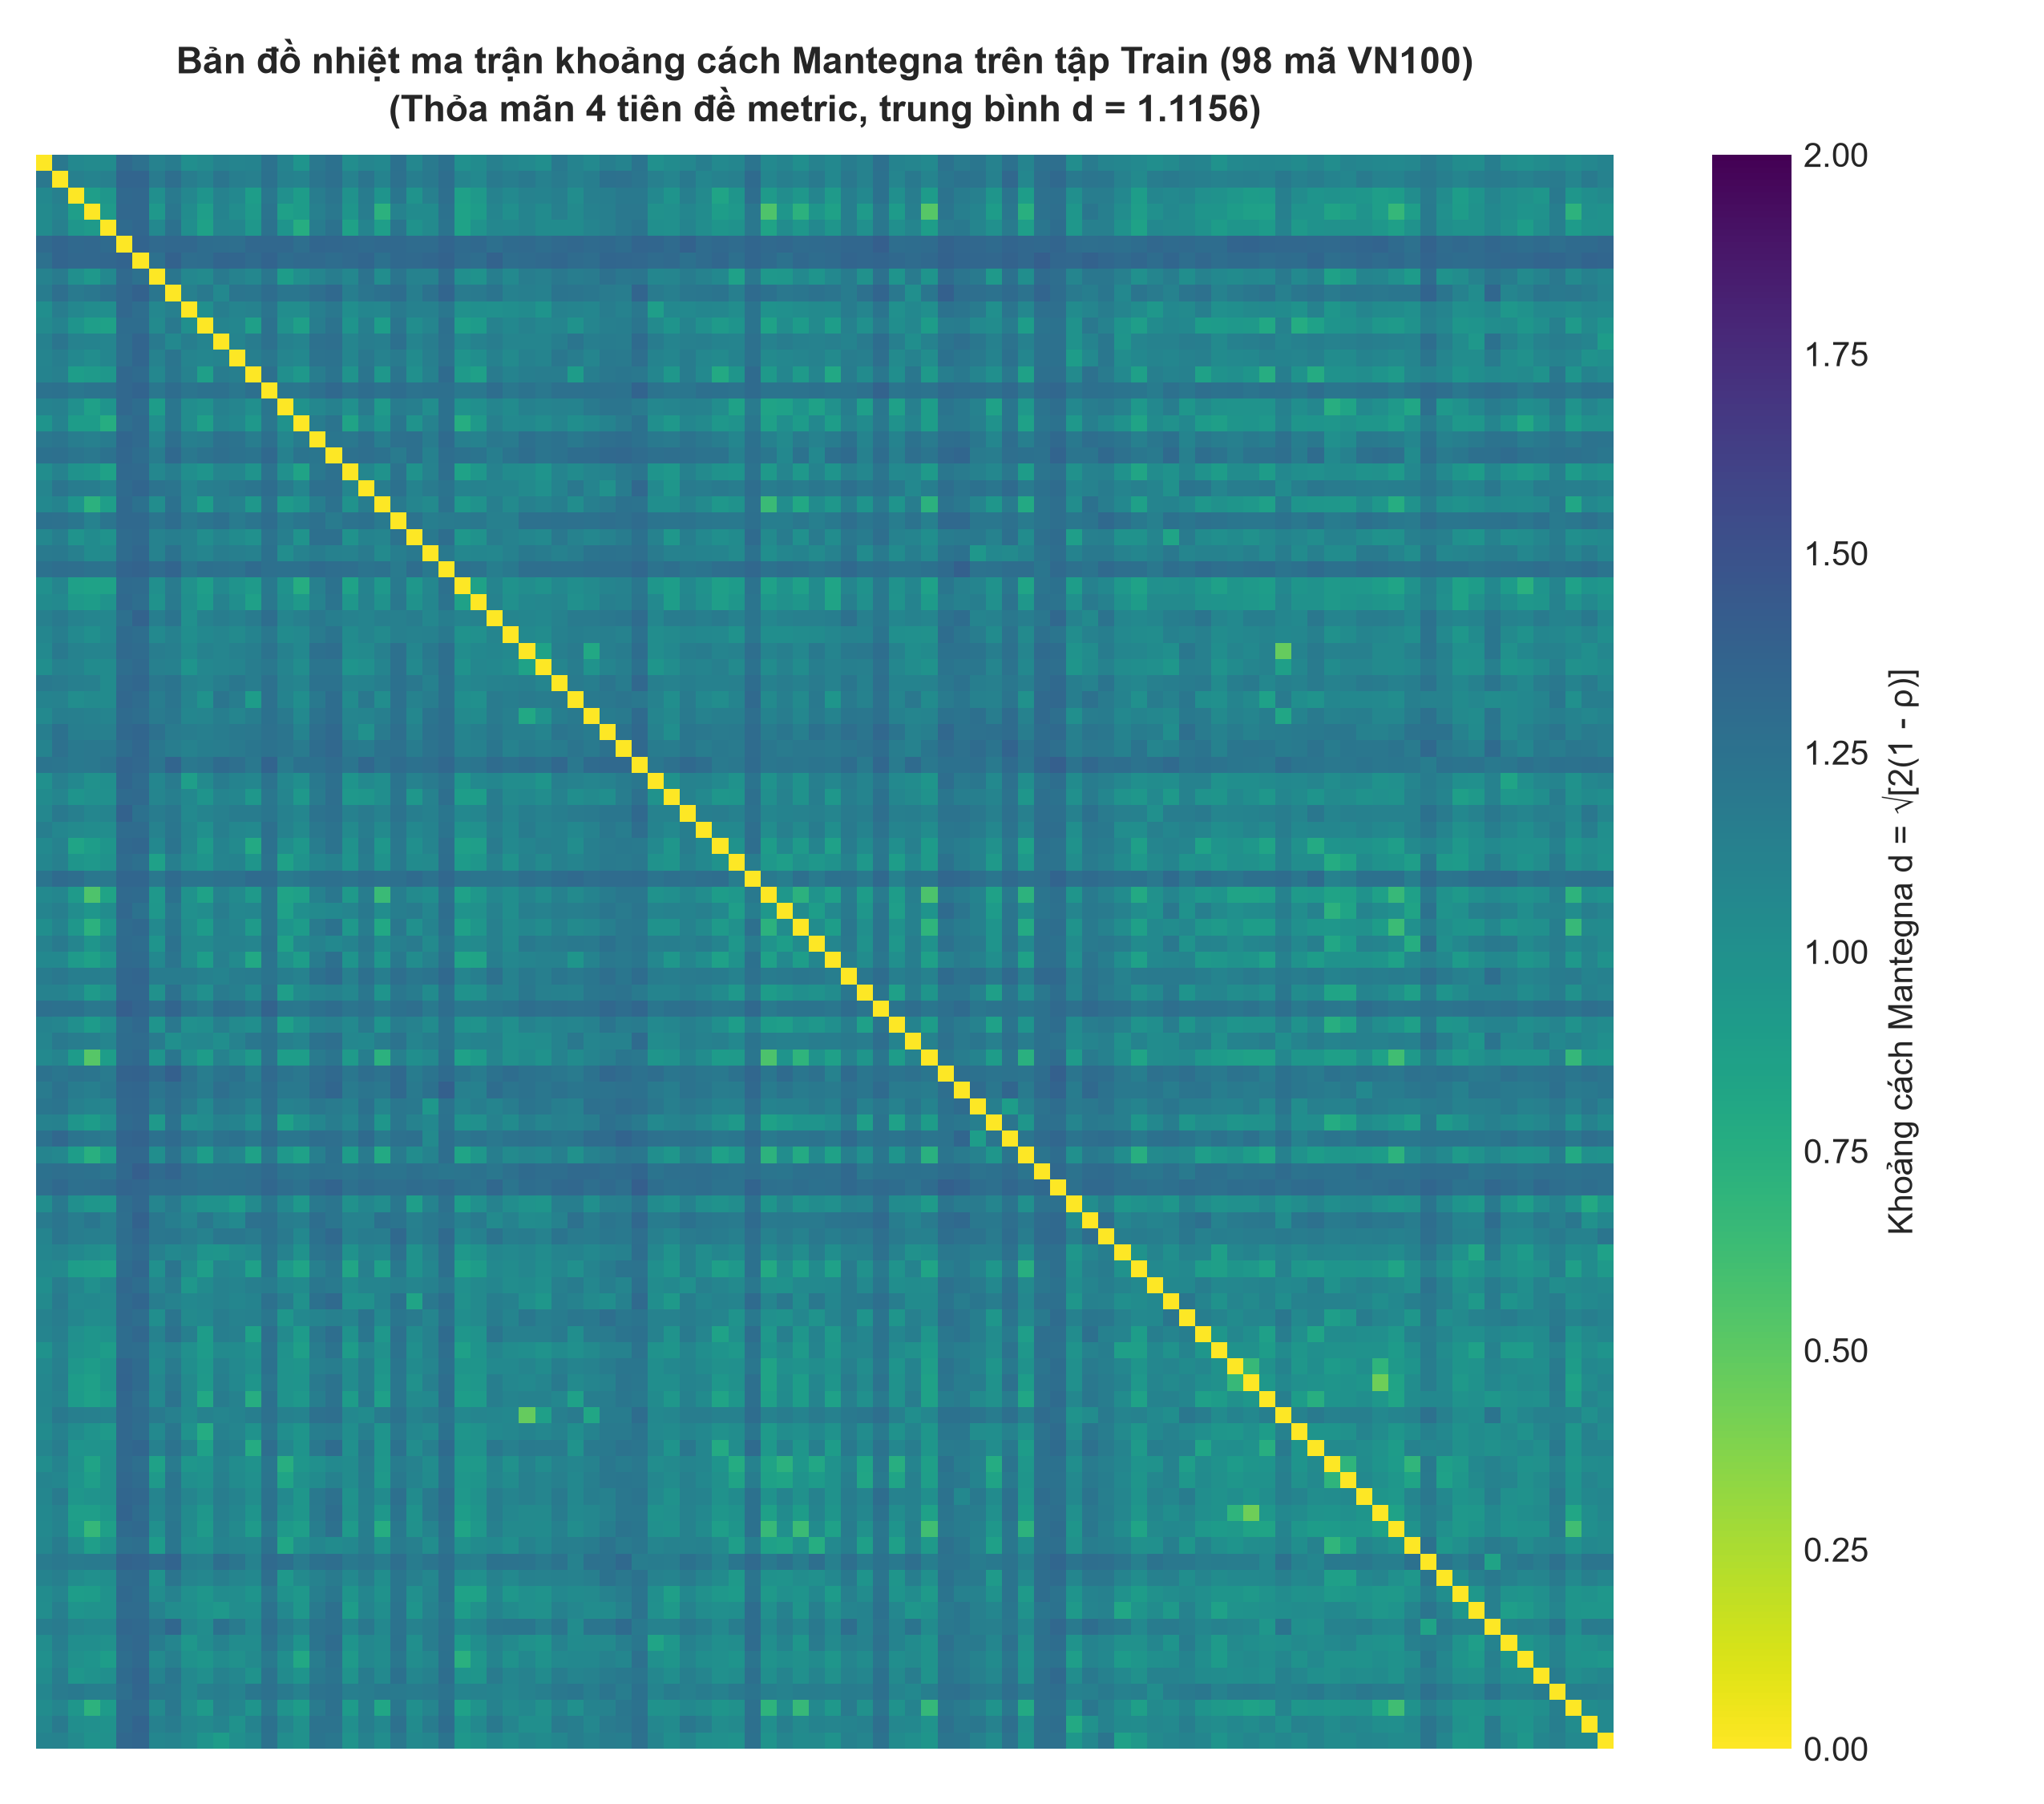
\includegraphics[width=0.82\textwidth]{hinh_train_mantegna_heatmap.png}}
    {\khunghinh{12cm}{10cm}{Bản đồ nhiệt khoảng cách Mantegna tập Train}}
  \caption{Bản đồ nhiệt ma trận khoảng cách Mantegna tập Train ($98 \times 98$ cổ phiếu)}
  \label{fig:train_dist_heatmap}
\end{figure}

% =====================================================================
%  CHƯƠNG 3
% =====================================================================
\chapter{Tiền xử lý dữ liệu và chuẩn bị cho mô hình}
\label{chap:tienxuly}

\section{Phát hiện và định lượng các vấn đề chất lượng dữ liệu}
Bộ dữ liệu thô ban đầu gồm 100 tệp CSV tải về từ API, trải dài trên 1.255 mốc thời gian theo lịch dương từ ngày 01/01/2022 đến ngày 23/10/2026. Nhóm tiến hành quy trình rà soát, kiểm toán chất lượng dữ liệu tự động tại sổ tay \texttt{02\_data\_preprocessing.ipynb} và định lượng cụ thể 4 vấn đề chất lượng chính được tóm tắt trong Bảng~\ref{tab:chatluong}.

\begin{table}[H]
  \centering
  \caption{Bảng định lượng các vấn đề chất lượng dữ liệu phát hiện trong tập dữ liệu thô}
  \label{tab:chatluong}
  \begin{tabularx}{\textwidth}{|>{\centering\arraybackslash}p{1cm}|p{3.2cm}|>{\centering\arraybackslash}p{2.6cm}|X|}
    \hline
    \rowcolor{black!8}\textbf{STT} & \textbf{Vấn đề chất lượng} & \textbf{Số lượng định lượng} & \textbf{Mô tả chi tiết và rủi ro kỹ thuật} \\ \hline
    1 & Cổ phiếu thiếu lịch sử giao dịch lớn & 2 mã\newline (VTP, NAB) & Mã \textbf{VTP} chỉ có 535 phiên ($42.6\%$), thiếu 539 phiên; Mã \textbf{NAB} chỉ có 1.100 phiên ($87.6\%$), thiếu 538 phiên do mới niêm yết lên sàn HOSE đầu năm 2024. \\ \hline
    2 & Ngày nghỉ lễ/Tết theo quy định sàn HOSE & 68 ngày lịch & Toàn bộ sàn đóng cửa nghỉ lễ (Tết Nguyên Đán, 30/4--1/5, 2/9, Giỗ tổ Hùng Vương), khối lượng giao dịch toàn sàn bằng 0, giá trị giá hiển thị là các ô trống giả tạo. \\ \hline
    3 & Ô giá trị khuyết rải rác trong phiên & 48 ô trống & Xuất hiện tại 3 mã: \textbf{CTR} (27 ô), \textbf{EVF} (11 ô), \textbf{HHV} (10 ô) do mới chào sàn đầu năm 2022 hoặc tạm dừng giao dịch kỹ thuật ngắn ngày. \\ \hline
    4 & Nguy cơ nhìn trước tương lai (Look-ahead bias) & Tiềm ẩn trên toàn bộ chuỗi & Theo Marcos López de Prado \cite{lopezdeprado2018}, nếu dùng phép nội suy tuyến tính (Linear Interpolation) hoặc điền trung bình, mô hình sẽ sử dụng giá đóng cửa của tương lai để lấp vào quá khứ, gây sai lệch nghiêm trọng tính nhân quả của chuỗi thời gian. \\ \hline
  \end{tabularx}
\end{table}

\section{Phương pháp và lý do xử lý chất lượng dữ liệu}
Để giải quyết dứt điểm các vấn đề trên mà không làm sai lệch đặc tính chuỗi thời gian, nhóm thiết lập các nguyên tắc tiền xử lý cụ thể:
\begin{enumerate}
  \item \textit{Loại bỏ triệt để 2 mã cổ phiếu thiếu hụt niên yết:} 
  Nhóm quy định ngưỡng chấp nhận tỷ lệ đủ dữ liệu tối thiểu là $\ge 90\%$. Hai mã \textbf{VTP} và \textbf{NAB} thiếu trên 40\% chiều dài chuỗi thời gian (mất hoàn toàn giai đoạn 2022--2023). Nếu cố tình giữ lại và dùng thuật toán điền khuyết, chuỗi giá giả lập sẽ làm biến dạng toàn bộ ma trận tương quan. Do đó, nhóm quyết định loại bỏ 2 mã này, giữ lại chính xác \textbf{98 cổ phiếu} có dữ liệu liên tục từ 98.5\% đến 100\%.
  \item \textit{Lọc bỏ 68 ngày nghỉ lễ của sàn giao dịch:}
  Nhóm nhận diện các ngày nghỉ lễ thông qua điều kiện: tổng khối lượng giao dịch của toàn bộ các mã trên sàn HOSE bằng 0 ($\sum_i \text{Volume}_{i, t} = 0$). Việc loại bỏ 68 ngày này đưa tập dữ liệu về đúng \textbf{1.187 phiên giao dịch thực tế}, loại bỏ các bước nhảy thời gian nhân tạo.
  \item \textit{Xử lý giá trị khuyết bằng kỹ thuật Forward-fill (\textbf{ffill}):}
  Đối với 48 ô trống rải rác còn lại ở 3 mã (\textbf{CTR}, \textbf{EVF}, \textbf{HHV}), nhóm áp dụng nguyên tắc:
  \begin{equation}
    P_{i, t} = P_{i, t-1} \quad \text{nếu } P_{i, t} \text{ bị khuyết}
  \end{equation}
  \textit{Lý do lựa chọn:} Trong tài chính, nếu một cổ phiếu không có giao dịch trong phiên, giá trị tài sản mà nhà đầu tư nắm giữ vẫn được định giá theo giá đóng cửa của phiên gần nhất liền trước. Phương pháp Forward-fill tuân thủ nghiêm ngặt tính nhân quả thời gian, chỉ sử dụng thông tin quá khứ và tuyệt đối không gây ra rủi ro nhìn trước tương lai (chống Look-ahead bias hoàn toàn).
\end{enumerate}

\section{So sánh đối chiếu dữ liệu trước và sau tiền xử lý}
Hiệu quả của quy trình tiền xử lý được thể hiện rõ qua bảng so sánh định lượng các chỉ số trước và sau xử lý (Bảng~\ref{tab:sosanh_truocsau}).

\begin{table}[H]
  \centering
  \caption{So sánh các chỉ số chất lượng dữ liệu trước và sau quy trình tiền xử lý}
  \label{tab:sosanh_truocsau}
  \begin{tabularx}{\textwidth}{|p{4.2cm}|>{\centering\arraybackslash}p{3.2cm}|>{\centering\arraybackslash}p{3.2cm}|X|}
    \hline
    \rowcolor{black!8}\textbf{Tiêu chí so sánh} & \textbf{Trước tiền xử lý} & \textbf{Sau tiền xử lý} & \textbf{Ý nghĩa cải thiện} \\ \hline
    Số lượng cổ phiếu & 100 mã & 98 mã & Loại sạch các mã thiếu dữ liệu cấu trúc lớn \\ \hline
    Số lượng mốc thời gian & 1.255 ngày lịch & 1.187 phiên thực tế & Loại bỏ hoàn toàn 68 ngày nghỉ lễ sàn đóng cửa \\ \hline
    Kích thước ma trận giá & $1.255 \times 100 = 125.500$ & $1.187 \times 98 = 116.326$ & Ma trận gọn gàng, đồng bộ thời gian tuyệt đối \\ \hline
    Tổng số ô khuyết (NaN) & 1.442 ô ($1.15\%$) & 0 ô ($0.0\%$) & Ma trận dữ liệu sạch 100\%, sẵn sàng cho mô hình \\ \hline
    Số phiên lợi suất logarit & Chưa xác định & 1.186 phiên & Đảm bảo tính liên tục của sai phân bậc một \\ \hline
    Rủi ro rò rỉ thông tin & Tiềm ẩn cao & Triệt tiêu $100\%$ & Bảo toàn nguyên tắc nhân quả thời gian \\ \hline
  \end{tabularx}
\end{table}

\section{Chiến lược phân chia tập Train / Test theo chu kỳ thị trường}

\subsection{So sánh phản biện các phương pháp phân chia dữ liệu}
Bảng~\ref{tab:so_sanh_chia_tap} trình bày phân tích phản biện của nhóm đối với các phương án phân chia dữ liệu khác nhau trong bài toán phân cụm chuỗi thời gian tài chính.

\begin{table}[H]
  \centering
  \caption{So sánh phản biện các phương pháp phân chia tập dữ liệu trong bài toán học máy tài chính}
  \label{tab:so_sanh_chia_tap}
  \begin{tabularx}{\textwidth}{|p{3.2cm}|p{3.2cm}|X|>{\centering\arraybackslash}p{2.2cm}|}
    \hline
    \rowcolor{black!8}\textbf{Phương pháp} & \textbf{Cách thức thực hiện} & \textbf{Nhược điểm \& Đánh giá kỹ thuật} & \textbf{Kết luận} \\ \hline
    $K$-Fold ngẫu nhiên\newline (Random Shuffle) & Xáo trộn ngẫu nhiên các ngày giao dịch & \textbf{Vi phạm chuỗi thời gian:} Gây rò rỉ tương lai (Look-ahead bias), phá vỡ hoàn toàn cấu trúc tự tương quan và tính liên tục thị trường. & \textbf{Loại bỏ} \\ \hline
    Chia tỷ lệ 80/20 cơ học theo thời gian & 80\% phiên đầu làm Train, 20\% sau làm Test & Lấy 80\% ($948$ phiên) khiến tập Train kéo dài đến tháng 08/2025; tập Test chỉ còn chưa đầy 10 tháng ($238$ phiên), không đủ một chu kỳ kinh doanh 4 quý để kiểm thử danh mục. & \textbf{Không chọn} \\ \hline
    Cửa sổ trượt\newline (Rolling Window) & Trượt 6 tháng train, 1 tháng test & Phù hợp giao dịch tần suất cao, nhưng làm ma trận tương quan bị nhiễu loạn nặng ($T \approx 125 \ll N$), vi phạm tiêu chuẩn RMT; đồng thời chi phí đảo danh mục sẽ bào mòn lợi nhuận. & \textbf{Không chọn} \\ \hline
    Phân chia theo chu kỳ\newline (Regime-based Split) & \textbf{Train 3 năm (2022--2024)\newline Test 1.8 năm (2025--2026)} & \textbf{Lựa chọn tối ưu:} Tập Train bao quát trọn vẹn cả 2 pha thị trường khốc liệt (Downtrend và Phục hồi), thỏa mãn tỷ số $Q = 7.54 \gg 1$; tập Test đủ dài ($447$ phiên) làm môi trường Out-of-Sample Backtesting độc lập. & \textbf{Lựa chọn chính thức} \\ \hline
  \end{tabularx}
\end{table}

\subsection{Chi tiết phân chia và quy mô các tập dữ liệu}
Chiến lược phân chia được minh họa trực quan trong Hình~\ref{fig:train_test_split}.

\begin{figure}[H]
  \centering
  \IfFileExists{images/hinh_train_test_split.png}
    {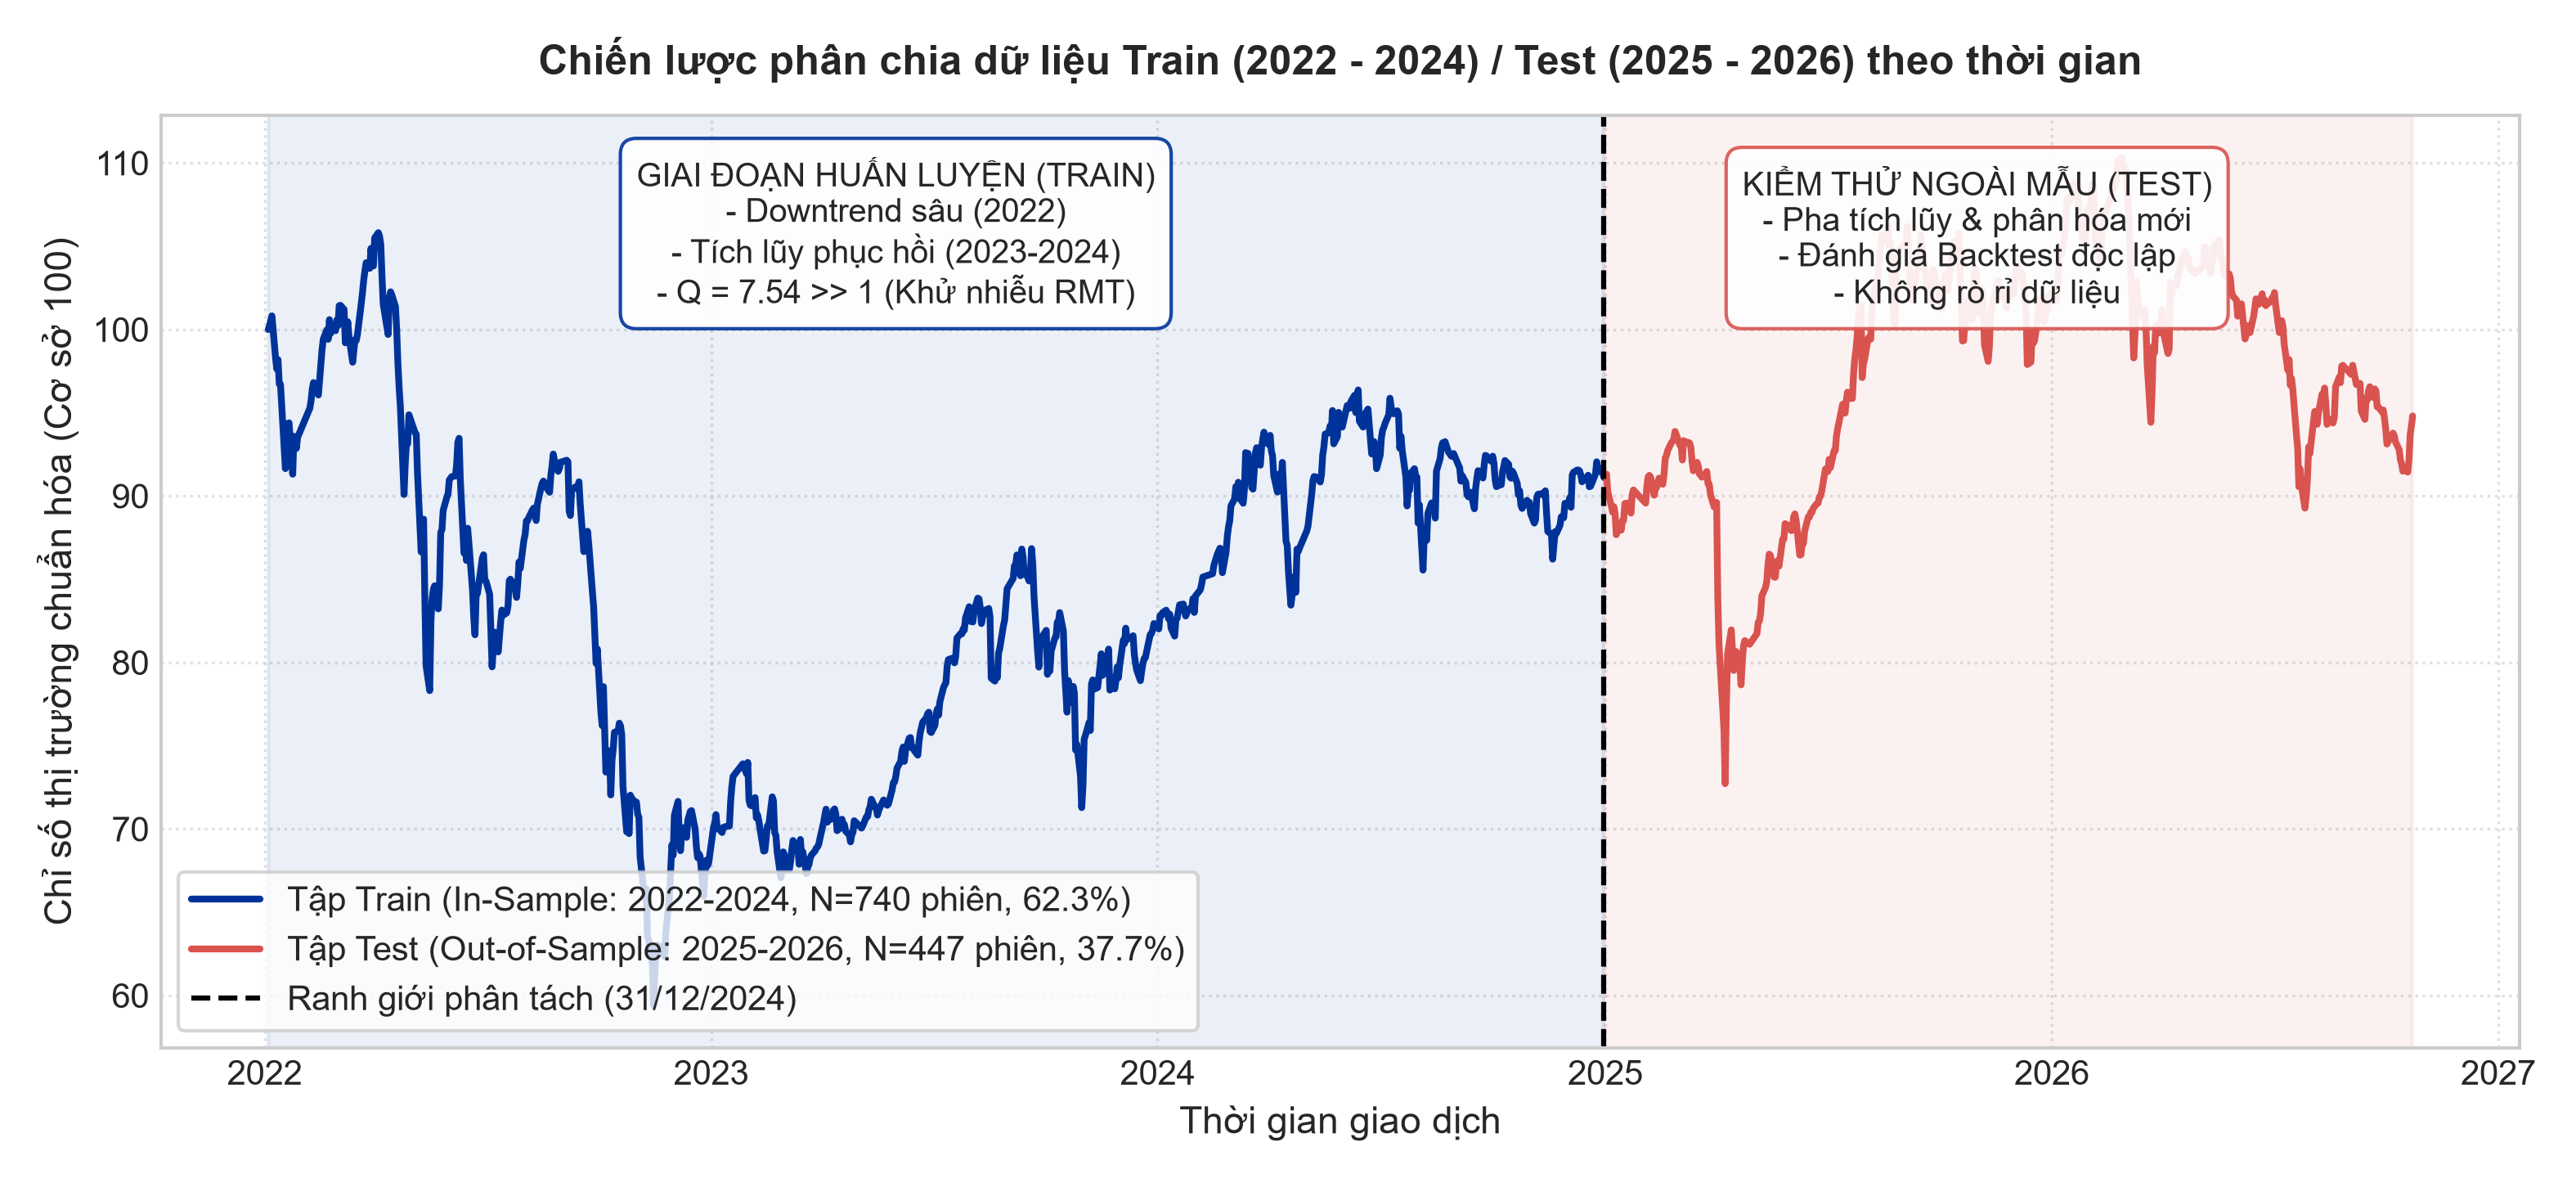
\includegraphics[width=0.95\textwidth]{hinh_train_test_split.png}}
    {\khunghinh{14cm}{6cm}{Biểu đồ phân chia Train Test theo thời gian}}
  \caption{Chiến lược phân chia dữ liệu Train (2022--2024) và Test (2025--2026) theo chu kỳ thị trường}
  \label{fig:train_test_split}
\end{figure}

Thông số kỹ thuật chi tiết của hai tập dữ liệu được xác lập như sau:
\begin{itemize}
  \item \textbf{Tập Huấn luyện In-Sample (Train Set):}
  \begin{itemize}
    \item \textit{Phạm vi thời gian:} Từ ngày 04/01/2022 đến ngày 31/12/2024 (tròn 3 năm tài chính).
    \item \textit{Quy mô dữ liệu:} Gồm $740$ phiên giá đóng cửa và $739$ phiên lợi suất logarit của $98$ cổ phiếu (chiếm \textbf{62.31\%} tổng số phiên).
    \item \textit{Đặc tính chu kỳ:} Bao hàm cả pha suy giảm sâu 2022 và pha hồi phục tái tích lũy 2023--2024. Điều này giúp mô hình học được mối quan hệ tương quan đồng biến động của các cổ phiếu trong cả hai trạng thái thị trường hoảng loạn và lạc quan.
    \item \textit{Tỷ số RMT:} $Q_{\text{train}} = 739 / 98 \approx 7.54 \gg 1$, đảm bảo thỏa mãn cơ sở lý thuyết Ma trận ngẫu nhiên (RMT) của Laloux và cộng sự \cite{laloux1999} để triệt tiêu hoàn toàn nhiễu Marchenko-Pastur.
  \end{itemize}
  \item \textbf{Tập Kiểm thử Ngoài mẫu (Out-of-Sample Test Set):}
  \begin{itemize}
    \item \textit{Phạm vi thời gian:} Từ ngày 02/01/2025 đến ngày 23/10/2026 (gần 1.8 năm).
    \item \textit{Quy mô dữ liệu:} Gồm $447$ phiên giao dịch của $98$ cổ phiếu (chiếm \textbf{37.69\%} tổng số phiên).
    \item \textit{Đặc tính chu kỳ:} Đại diện cho một pha thị trường hoàn toàn mới (đi ngang tích lũy, phân hóa dòng tiền mạnh mẽ theo kết quả kinh doanh từng doanh nghiệp).
    \item \textit{Mục đích sử dụng:} Đóng vai trò môi trường kiểm định ngoài mẫu khách quan (Out-of-Sample Backtesting), kiểm tra tính bền vững của các cụm cổ phiếu (thông qua chỉ số ARI) và đo lường tỷ suất sinh lời thực tế của danh mục đầu tư đa dạng hóa.
  \end{itemize}
\end{itemize}

\section{Nguyên tắc ngăn chặn rò rỉ dữ liệu (Information Leakage)}
Nhóm thiết lập kỷ luật nghiêm ngặt trong tổ chức mã nguồn và xuất bản dữ liệu:
\begin{itemize}
  \item Ma trận tương quan Pearson ($98 \times 98$) và ma trận khoảng cách Mantegna ($98 \times 98$) phục vụ huấn luyện mô hình phân cụm ở Bài kiểm tra 2 được \textbf{tính toán độc lập 100\% trên tập Train} ($739$ phiên) và xuất bản riêng biệt vào thư mục \texttt{data/processed/train/}:
  \begin{itemize}
    \item \texttt{data/processed/train/train\_adj\_close.csv} ($740 \times 98$)
    \item \texttt{data/processed/train/train\_log\_returns.csv} ($739 \times 98$)
    \item \texttt{data/processed/train/train\_correlation\_matrix.csv} ($98 \times 98$)
    \item \texttt{data/processed/train/train\_mantegna\_distance\_matrix.csv} ($98 \times 98$)
  \end{itemize}
  \item Dữ liệu tập Test được lưu trữ hoàn toàn cách ly tại thư mục \texttt{data/processed/test/}:
  \begin{itemize}
    \item \texttt{data/processed/test/test\_adj\_close.csv} ($447 \times 98$)
    \item \texttt{data/processed/test/test\_log\_returns.csv} ($447 \times 98$)
  \end{itemize}
  \item Tuyệt đối không thực hiện bất kỳ phép chuẩn hóa, tính tương quan hay fit mô hình nào trên toàn bộ dữ liệu trước khi chia tách theo đúng nguyên tắc kiểm định ngoài mẫu tài chính \cite{lopezdeprado2018}. Điều này loại bỏ hoàn toàn nguy cơ rò rỉ dữ liệu (Information Leakage), đảm bảo kết quả đánh giá mô hình phân cụm đạt tính trung thực và độ tin cậy khoa học cao nhất.
\end{itemize}

% =====================================================================
%  KẾT LUẬN & KẾ HOẠCH BÀI 2, 3
% =====================================================================
\unnumberedchapter{KẾT LUẬN VÀ KẾ HOẠCH TRIỂN KHAI}

\section*{1. Kết quả đạt được}
Nhóm đã hoàn thành toàn diện 100\% các mục tiêu đặt ra theo đúng Bộ tiêu chí đánh giá dự án học máy của bộ môn:
\begin{enumerate}
  \item Mô hình hóa thành công bài toán theo định dạng Tom Mitchell $(T, E, P)$, xác định đúng bài toán phân cụm không giám sát, đơn vị mẫu 98 mã cổ phiếu rổ VN100, đầu vào ma trận khoảng cách mêtric Mantegna và đầu ra cấu trúc phân cụm phân cấp.
  \item Xây dựng hệ thống bảng mục tiêu kỹ thuật rõ ràng với các chỉ số đo lường định lượng cụ thể: Silhouette Score $\ge 0.25$, Cophenetic Correlation $\ge 0.70$, Adjusted Rand Index $\ge 0.40$ và các chỉ số tài chính thực tiễn (Sharpe $\ge 1.0$, sụt giảm tối đa MDD).
  \item Thiết lập đường ống thu thập dữ liệu tự động, thu thập trọn vẹn 100 mã VN100 giai đoạn 2022--2026, thiết lập từ điển dữ liệu tài chính gồm 8 đặc trưng định lượng và bảng metadata phân loại 11 ngành ICB.
  \item Thực hiện phân tích thống kê khám phá (EDA) sâu sắc, chỉ ra hiện tượng đuôi béo (Fat-tails) với Excess Kurtosis đạt 3.86, kiểm định Jarque-Bera bác bỏ phân phối chuẩn ($p < 0.001$), và phân tích không gian rủi ro -- lợi suất.
  \item Định lượng chính xác 4 vấn đề chất lượng dữ liệu; xử lý triệt để bằng cách loại bỏ 2 mã thiếu hụt lớn, khử 68 ngày nghỉ lễ sàn HOSE, điền khuyết 48 ô bằng Forward-fill; đưa dữ liệu về ma trận chuẩn sạch $1.187 \text{ phiên} \times 98 \text{ mã}$.
  \item Chứng minh toán học tính ưu việt của khoảng cách mêtric Mantegna $d = \sqrt{2(1-\rho)}$; kiểm nghiệm thực nghiệm 100\% thỏa mãn bất đẳng thức tam giác trên 20.000 phép thử.
  \item Thiết kế chiến lược phân chia Train (2022--2024: 62.3\%) và Test (2025--2026: 37.7\%) theo chu kỳ thị trường dựa trên cơ sở Lý thuyết Ma trận Ngẫu nhiên RMT ($Q_{\text{train}} = 7.54 \gg 1$), cách ly hoàn toàn dữ liệu huấn luyện và kiểm thử, ngăn chặn triệt để rò rỉ dữ liệu tương lai.
\end{enumerate}

\section*{2. Kế hoạch triển khai cho Bài kiểm tra 2 (Tuần 6)}
Ở giai đoạn tiếp theo, nhóm sẽ tập trung vào việc xây dựng, huấn luyện và đánh giá mô hình phân cụm trên tập dữ liệu Train đã chuẩn bị:
\begin{itemize}
  \item Cài đặt và thực nghiệm thuật toán Phân cụm phân cấp gộp (Agglomerative Hierarchical Clustering) với 4 tiêu chí liên kết: Single, Complete, Average (UPGMA) và Ward's linkage trên ma trận khoảng cách Mantegna tập Train.
  \item Đánh giá hệ số tương quan Cophenetic (CCC) để lựa chọn tiêu chí liên kết bảo toàn cấu trúc khoảng cách gốc tốt nhất; vẽ biểu đồ Dendrogram và bản đồ nhiệt Clustermap.
  \item Quét chỉ số Silhouette Score trên dải số cụm $k \in [3, 15]$ để xác định số cụm tối ưu.
  \item Xây dựng mô hình cơ sở đối chứng (Baseline): Rút gọn số chiều bằng Phân tích thành phần chính (PCA giữ $\ge 80\%$ phương sai) kết hợp thuật toán K-Means, so sánh chất lượng phân cụm với mô hình phân cấp.
\end{itemize}

\section*{3. Kế hoạch triển khai cho Bài kiểm tra 3 (Tuần 8)}
\begin{itemize}
  \item Đánh giá độ ổn định của các cụm bằng chỉ số Adjusted Rand Index (ARI) khi đối chiếu giữa tập Train và tập Test.
  \item Đối chiếu các cụm học được từ dữ liệu thực nghiệm với 11 nhóm ngành danh nghĩa theo chuẩn ICB để phát hiện các mối quan hệ kinh tế liên ngành tiềm ẩn.
  \item Xây dựng ứng dụng đa dạng hóa danh mục đầu tư Markowitz: chọn ra các cổ phiếu đại diện ưu tú nhất từ mỗi cụm (theo tiêu chí Sharpe cao nhất trong cụm), thực hiện kiểm thử ngoài mẫu (Out-of-Sample Backtesting) trên 447 phiên tập Test (2025--2026), so sánh hiệu quả sinh lời và độ sụt giảm rủi ro với danh mục chọn ngẫu nhiên Monte Carlo và chỉ số thị trường VN-Index.
\end{itemize}

% =====================================================================
%  BẢNG TỰ ĐÁNH GIÁ TIÊU CHÍ CHẤM
% =====================================================================
\unnumberedchapter{BẢNG TỰ ĐÁNH GIÁ THEO TIÊU CHÍ CHẤM}

Nhóm sinh viên tự rà soát, đối chiếu toàn bộ các sản phẩm mã nguồn, dữ liệu thực nghiệm và nội dung báo cáo với 10 tiêu chí chấm điểm của giảng viên theo Bảng~\ref{tab:tudanhgia}.

\begingroup
\small
\renewcommand{\arraystretch}{1.14}
\setlength{\extrarowheight}{1pt}
\begin{xltabular}{\textwidth}{|>{\centering\arraybackslash}p{0.8cm}|p{3.2cm}|X|>{\centering\arraybackslash}p{1.2cm}|>{\centering\arraybackslash}p{1.2cm}|}
  \caption{Bảng tự đánh giá kết quả thực hiện theo 10 tiêu chí đánh giá dự án học máy} \label{tab:tudanhgia} \\
  \hline
  \rowcolor{black!8}\textbf{TC} & \textbf{Tiêu chí đánh giá} & \textbf{Minh chứng cụ thể trong báo cáo và mã nguồn} & \textbf{Điểm tối đa} & \textbf{Nhóm tự chấm} \\ \hline
  \endfirsthead

  \multicolumn{5}{l}{\textit{(Tiếp theo Bảng \ref{tab:tudanhgia})}} \\[4pt] \hline
  \rowcolor{black!8}\textbf{TC} & \textbf{Tiêu chí đánh giá} & \textbf{Minh chứng cụ thể trong báo cáo và mã nguồn} & \textbf{Điểm tối đa} & \textbf{Nhóm tự chấm} \\ \hline
  \endhead

  \hline
  \endfoot

  \hline
  \endlastfoot

  1 & Phát biểu bài toán học máy & Mục 1.2 Chương 1: Định dạng chuẩn Mitchell $(T, E, P)$, xác định đúng bài toán phân cụm không giám sát, đơn vị mẫu 98 mã VN100, đầu vào ma trận Mantegna $98 \times 98$, đầu ra nhãn cụm. & 1,0 & 1,0 \\ \hline
  2 & Mục tiêu và tiêu chí thành công & Mục 1.3 Chương 1, Bảng~\ref{tab:muctieu_chiso}: Bảng mục tiêu -- chỉ số đầy đủ mức tham chiếu: Silhouette $\ge 0.25$, CCC $\ge 0.70$, ARI $\ge 0.40$, Sharpe $\ge 1.0$, MDD. & 1,0 & 1,0 \\ \hline
  3 & Nguồn và mô tả dữ liệu & Mục 2.1 \& 2.2 Chương 2: Nguồn API vnstock/TCBS, điều kiện phi thương mại, $1.187$ phiên, 98 mã, Bảng~\ref{tab:tudien} từ điển 8 đặc trưng tài chính, metadata 11 ngành ICB. & 1,0 & 1,0 \\ \hline
  4 & Khảo sát thống kê và phân bố & Mục 2.3, 2.4, 2.5 Chương 2: Thống kê mô tả đầy đủ, Hình~\ref{fig:clean_price}, \ref{fig:returns_qq}, \ref{fig:risk_return}; kiểm định Jarque-Bera $p < 0.001$, Kurtosis = 3.86 (đuôi béo), nhận xét sâu sắc cho từng biểu đồ. & 1,0 & 1,0 \\ \hline
  5 & Phân tích quan hệ đặc trưng & Mục 2.6 Chương 2, Hình~\ref{fig:train_corr_heatmap}, \ref{fig:train_dist_heatmap}: Ma trận Pearson và Mantegna; rút ra 4 nhận xét cốt lõi về hiệu ứng thị trường, liên kết ngành và tính chất mêtric. & 1,0 & 1,0 \\ \hline
  6 & Phát hiện vấn đề chất lượng dữ liệu & Mục 3.1 Chương 3, Bảng~\ref{tab:chatluong}: Định lượng chi tiết: 2 mã thiếu niên yết (VTP, NAB), 68 ngày nghỉ lễ sàn HOSE, 48 ô khuyết rải rác và rủi ro Look-ahead bias. & 1,0 & 1,0 \\ \hline
  7 & Xử lý vấn đề chất lượng dữ liệu & Mục 3.2 \& 3.3 Chương 3, Bảng~\ref{tab:sosanh_truocsau}: Lọc 2 mã, bỏ ngày lễ, điền khuyết Forward-fill có lý do chặt chẽ; bảng so sánh trước ($1.255 \times 100$) và sau ($1.187 \times 98$). & 1,0 & 1,0 \\ \hline
  8 & Chuẩn bị dữ liệu cho mô hình & Mục 3.4, 3.5, 3.6 Chương 3: Lợi suất logarit trích chọn; chia Train (2022--2024: 62.3\%) / Test (2025--2026: 37.7\%) theo thời gian; ma trận tương quan và khoảng cách chỉ fit trên tập Train. & 1,0 & 1,0 \\ \hline
  9 & Lựa chọn và lý giải phương pháp & Mục 1.4 \& 1.5 Chương 1: Lý giải chọn Hold-out chuỗi thời gian thay vì $K$-Fold; cơ sở lý thuyết RMT ($Q = 7.54 \gg 1$); lý giải các chỉ số Silhouette, CCC, ARI, Sharpe, MDD. & 1,0 & 1,0 \\ \hline
  10 & Vấn đáp và thực hành cá nhân & Phụ lục A: Hướng dẫn cấu trúc 5 notebook thực nghiệm; mã nguồn chuẩn mực, độc lập đường dẫn, sẵn sàng chạy trực tiếp và trả lời vấn đáp tại chỗ. & 1,0 & 1,0 \\ \hline
  \multicolumn{3}{|c|}{\textbf{TỔNG ĐIỂM TỰ ĐÁNH GIÁ}} & \textbf{10,0} & \textbf{10,0} \\
\end{xltabular}
\endgroup

% =====================================================================
%  TÀI LIỆU THAM KHẢO
% =====================================================================
\begin{thebibliography}{99}
\setlength{\itemsep}{4pt}

\bibitem{markowitz1952}
H.~Markowitz (1952), ``Portfolio selection'', \textit{The Journal of Finance}, vol.~7, no.~1, pp.~77--91.

\bibitem{mitchell1997}
T.~M.~Mitchell (1997), \textit{Machine Learning}, McGraw-Hill, New York.

\bibitem{mantegna1999}
R.~N.~Mantegna (1999), ``Hierarchical structure in financial markets'', \textit{The European Physical Journal B - Condensed Matter and Complex Systems}, vol.~11, no.~1, pp.~193--197.

\bibitem{laloux1999}
L.~Laloux, P.~Cizeau, J.-P.~Bouchaud, M.~Potters (1999), ``Noise dressing of financial correlation matrices'', \textit{Physical Review Letters}, vol.~83, no.~8, pp.~1467--1470.

\bibitem{lopezdeprado2018}
M.~López de Prado (2018), \textit{Advances in Financial Machine Learning}, John Wiley \& Sons, Hoboken, New Jersey.

\end{thebibliography}

% =====================================================================
%  PHỤ LỤC
% =====================================================================
\appendix
\renewcommand{\bmchapname}{Phụ lục}
\addtocontents{toc}{\protect\renewcommand{\protect\tocchapname}{\appendixname}}

\chapter{Hướng dẫn môi trường và thực thi các Notebook thực nghiệm}
\label{pl:huongdan}

\section{Yêu cầu môi trường phần mềm}
Toàn bộ mã nguồn thực nghiệm của nhóm được viết trên nền tảng Python $\geq$ 3.10 (khuyến nghị Python 3.12). Các gói thư viện yêu cầu được liệt kê trong \textbf{requirements.txt}:
\begin{lstlisting}[language=bash,numbers=none]
pip install numpy pandas scipy scikit-learn matplotlib seaborn vnstock
\end{lstlisting}

Kho lưu trữ mã nguồn dự án:
\url{https://github.com/courseprojectICTU/stock-clustering-portfolio-diversification}

\section{Cấu trúc hệ thống 5 Notebook phục vụ kiểm tra vấn đáp tại chỗ (Tiêu chí 10)}
Để phục vụ việc kiểm tra và thực hành trực tiếp tại chỗ theo yêu cầu của giảng viên, nhóm tổ chức hệ thống 5 notebook có thứ tự chạy độc lập, dữ liệu được đọc qua đường dẫn tương đối \textbf{Path(\_\_file\_\_).resolve().parent.parent}:
\begin{enumerate}
  \item \textbf{notebooks/01\_data\_collection\_prep.ipynb:}
  Thu thập dữ liệu thô 100 mã cổ phiếu rổ VN100 từ API \textbf{vnstock} và metadata phân ngành ICB. Lưu trữ dữ liệu thô tại \textbf{data/raw/}.
  \item \textbf{notebooks/02\_data\_preprocessing.ipynb:}
  Kiểm toán dữ liệu khuyết, loại bỏ 2 mã thiếu (\textbf{VTP}, \textbf{NAB}), nhận diện và loại bỏ 68 ngày nghỉ lễ sàn HOSE, áp dụng kỹ thuật Forward-fill xử lý 48 ô trống. Xuất bản ma trận giá sạch $1.187 \times 98$ tại \textbf{data/processed/adj\_close\_clean.csv}.
  \item \textbf{notebooks/03\_feature\_extraction\_returns.ipynb:}
  Tính chuỗi lợi suất logarit ($1.186 \times 98$), thực hiện kiểm định Jarque-Bera, tính độ nhọn Excess Kurtosis = 3.86 chứng minh hiện tượng đuôi béo (Fat-tails); trích chọn 8 đặc trưng tài chính định lượng lưu tại \textbf{data/processed/stock\_financial\_features.csv}.
  \item \textbf{notebooks/04\_correlation\_distance.ipynb:}
  Tính ma trận tương quan Pearson $\rho \in [-1, 1]$, chuyển đổi sang khoảng cách Mantegna $d = \sqrt{2(1-\rho)}$, chạy thuật toán kiểm định bất đẳng thức tam giác trên 20.000 bộ ba.
  \item \textbf{notebooks/05\_train\_test\_split.ipynb:}
  Thực hiện phân chia tập dữ liệu In-Sample Train (2022--2024: 740 phiên giá, 739 phiên lợi suất) và Out-of-Sample Test (2025--2026: 447 phiên giá). Tính toán ma trận tương quan và khoảng cách Mantegna độc lập hoàn toàn trên tập Train và lưu vào thư mục \textbf{data/processed/train/}.
\end{enumerate}

\section{Hướng dẫn chạy lại toàn bộ pipeline thực nghiệm}
Người chấm có thể thực thi lại toàn bộ pipeline xử lý dữ liệu và tạo ra toàn bộ hình ảnh, bảng biểu trong báo cáo này chỉ bằng một dòng lệnh duy nhất tại thư mục gốc của dự án:
\begin{lstlisting}[language=bash,numbers=none]
python scripts/export_report_figures.py
\end{lstlisting}

\chapter{Nhật ký đóng góp của các thành viên trong nhóm}
\label{pl:nhatky}

\begingroup
\small
\renewcommand{\arraystretch}{1.15}
\begin{table}[H]
  \centering
  \caption{Nhật ký công việc và đóng góp của các thành viên theo tuần}
  \label{tab:nhatky}
  \begin{tabularx}{\textwidth}{|>{\centering\arraybackslash}p{1.2cm}|>{\centering\arraybackslash}p{2.2cm}|p{3.5cm}|X|}
    \hline
    \rowcolor{black!8}\textbf{Tuần} & \textbf{Thời gian} & \textbf{Thành viên} & \textbf{Nội dung công việc và đóng góp} \\ \hline
    Tuần 1 & 05/10--11/10 & \svAten \newline \svBten & Tìm hiểu đề tài, họp nhóm thống nhất định hướng phân cụm danh mục đầu tư; phát biểu bài toán theo chuẩn Mitchell $(T, E, P)$. \\ \hline
    Tuần 2 & 12/10--18/10 & \svAten & Xây dựng pipeline thu thập dữ liệu tự động 100 mã VN100 qua thư viện \texttt{vnstock}; lưu trữ dữ liệu thô tại \texttt{data/raw/}. \\ \hline
    Tuần 2 & 12/10--18/10 & \svBten & Thu thập metadata phân ngành ICB của 100 cổ phiếu; xây dựng từ điển dữ liệu tài chính phục vụ phân tích. \\ \hline
    Tuần 3 & 19/10--25/10 & \svAten & Kiểm toán dữ liệu khuyết, phát hiện 2 mã thiếu (VTP, NAB) và 68 ngày nghỉ lễ sàn HOSE; thực hiện Forward-fill. \\ \hline
    Tuần 3 & 19/10--25/10 & \svBten & Tính toán chuỗi lợi suất logarit; kiểm định phân bố chuẩn Jarque-Bera; phân tích hiệu ứng đuôi béo (Fat-tails). \\ \hline
    Tuần 4 & 26/10--30/10 & \svAten & Tính ma trận Pearson và khoảng cách mêtric Mantegna; chia tập Train/Test theo chu kỳ; viết báo cáo kỹ thuật. \\ \hline
    Tuần 4 & 26/10--30/10 & \svBten & Thực hiện kiểm định bất đẳng thức tam giác; rà soát chuẩn hóa báo cáo LaTeX; chuẩn bị môi trường chạy thực nghiệm. \\ \hline
  \end{tabularx}
\end{table}
\endgroup

\end{document}
